
\part{Modéliser la langue}

\section*{Présentation}

Cette première partie est consacrée à la modélisation des langues en général. Elle est divisée en trois chapitres. Le premier chapitre essaye de définir la langue, notre objet d’étude, et précise les caractéristiques que nous retenons dans notre modélisation. Le deuxième chapitre montre à travers l’étude de la production d’un énoncé où se situent la syntaxe et la grammaire dans un modèle complet de la langue. Le troisième chapitre caractérise le type de modèles que nous adoptons dans cet ouvrage.

\chapter{\gkchapter{La langue}{L’objet d’étude de la linguistique}}\label{sec:1.1}

\section{Parler une langue}\label{sec:1.1.0}

Pour comprendre ce qu’est une langue, il faut comprendre à quoi elle sert. Savoir \textbf{utiliser une langue}, c’est être capable de parler dans cette langue et de comprendre ceux qui nous parlent. \textbf{Parler une langue}, c’est être capable de verbaliser n’importe quelle idée, c’est-à-dire \textbf{transformer un sens en un son} dont notre interlocuteur pourra lui-même extraire un sens (voir dans l’encadré qui suit le schéma proposé par Saussure). Si le sens de départ – celui pensé par le locuteur – et le sens d’arrivée – celui construit par le destinataire – sont suffisamment proches, alors, la \textbf{communication} peut être considérée comme réussie.

La \textstyleTermes{langue} est donc avant tout un objet qui se trouve dans le \textbf{cerveau} des locuteurs et que l’on peut modéliser par une \textbf{correspondance entre des sens et des sons}. Plus exactement, nous modélisons la langue par une correspondance entre des représentations sémantiques et des textes. Dans la suite, nous utiliserons le terme \textstyleTermes{texte} pour désigner les productions langagières qu’elles soient orales, écrites ou gestuelles. Ce terme a l’avantage de ne pas présupposer quelle est la nature du médium utilisé pour communiquer. Il a également l’avantage sur le terme \textit{son} de renvoyer à une représentation du son et non au son lui-même. Un texte sonore est ainsi la représentation que nous avons du son dans notre cerveau lorsque nous produisons des sons afin de communiquer. L’étude même de la représentation du son — la \textstyleTermes{phonologie} — ne sera abordée que dans la mesure où elle interfère avec la syntaxe. Nous nous intéressons à la modélisation du mécanisme cognitif (situé dans le cerveau) et nous laissons de côté le mécanisme physique qui permet la production du son à partir du texte (cela concerne la phonétique articulatoire), ainsi que le mécanisme auditif qui permet le décodage du son.

Considérer que la langue est une correspondance, c’est faire abstraction des mécanismes propres à la production ou la compréhension d’un texte. Le locuteur utilise la correspondance du sens vers le texte, tandis que le destinataire effectue le chemin inverse. Nous supposons implicitement que les deux directions, sens vers texte et texte vers sens, utilisent le même ensemble de connaissances et un mécanisme commun, qui constituent la langue proprement dite.

\chevalier{La langue comme correspondance sens-texte}{
    On trouve déjà dans le \textit{Cours de linguistique générale} de Ferdinand de Saussure, publié en 1916, la conception de la langue comme un objet qui fait se correspondre des sens et des «~sons~». Voici ce qu’il écrit :

    \begin{quote}
    «~Pour trouver dans l’ensemble du langage la sphère qui correspond à la langue, il faut se placer devant l’acte individuel qui permet de reconstituer le circuit de la parole. Cet acte suppose au moins deux individus ; c’est le minimum exigible pour que le circuit soit complet. Soient donc deux personnes A et B, qui s’entretiennent :

%     \begin{figure}
%     \caption{\label{fig:}}
    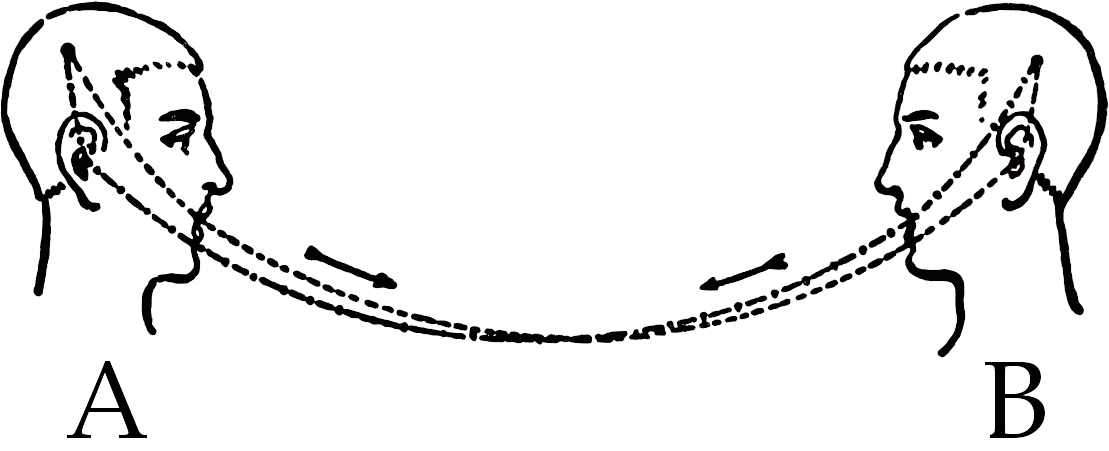
\includegraphics[width=\textwidth]{figures/vol1syntaxe2-img011.png}
%     \end{figure}

    Le point de départ du circuit est dans le cerveau de l’une, par exemple A, où les faits de conscience, que nous appellerons concepts, se trouvent associés aux représentations des signes linguistiques ou images acoustiques servant à leur expression. Supposons qu’un concept donné déclenche dans le cerveau une image acoustique correspondante : c’est un phénomène entièrement \textit{psychique}, suivi à son tour d’un procès \textit{physiologique} : le cerveau transmet aux organes de la phonation une impulsion corrélative à l’image ; puis les ondes sonores se propagent de la bouche de A à l’oreille de B : procès purement \textit{physique}. Ensuite, le circuit se prolonge en B dans un ordre inverse : de l’oreille au cerveau, transmission physiologique de l’image acoustique ; \textbf{dans le cerveau association psychique de cette image psychique avec le concept correspondant}. Si B parle à son tour ce nouvel acte suivra — de son cerveau à celui de A — exactement la même marche que le premier et passera par les mêmes phases successives.~» (\citealt{Saussure1916} : 27-28) [c’est nous qui soulignons]
    \end{quote}

    Saussure insiste, quelques lignes plus loin, sur le fait que l’association entre sens et son qui a lieu dans le cerveau ne se fait pas avec le son lui-même, mais avec une représentation de ce son dans le cerveau, que Saussure nomme l’\textbf{image acoustique~}:

    \begin{quote}
    «~[Il faut] distinguer les parties physiques (ondes sonores) des physiologiques (phonation et audition) et psychiques (images verbales et concepts). Il est en effet capital de remarquer que l’image verbale ne se confond pas avec le son lui-même et qu’elle est psychique au même titre que le concept qui lui est associé.~» (\citealt{Saussure1916} : 28-29)
    \end{quote}

    Leonard \citet[27]{Bloomfield1933}, le père de la linguistique américaine, va dans le même sens :

    \begin{quote}
    «~On produit de nombreuses sortes de bruits vocaux dont on utilise la variété : sous certains types de stimuli, on produit certains sons vocaux et nos compagnons, entendant les mêmes sons, font la réponse appropriée. Pour le dire brièvement, dans la parole humaine, des sons différents ont des sens différents. \textbf{Étudier} \textbf{la coordination de certains sons avec certains sens,} \textbf{c’est} \textbf{étudier la langue.}~» [nous soulignons]
    \end{quote}

    Le fait de considérer que l’objet d’étude de la linguistique est de modéliser la correspondance sens-son décrite par Saussure (et appelée par lui association concept-image acoustique) peut être imputé à Žolkovskij et Mel’čuk qui posent en 1967 à Moscou les bases de la Théorie Sens-Texte, dont le nom même est tout à fait explicite sur ce point. Dans son cours au Collège de France en 1997 intitulé \textit{Vers une linguistique Sens-Texte}, Igor Mel’čuk pose qu’un modèle d’une langue est une correspondance multivoque entre un ensemble de sens et un ensemble de textes, où les textes désignent les images acoustiques des phrases de la langue. Le caractère multivoque est dû au fait qu’un même sens peut être exprimé par différents textes (qui sont alors des «~paraphrases~» les uns des autres) et qu’un texte peut avoir plusieurs sens (c’est-à-dire être sémantiquement ambigu).

    Cette conception de la langue comme une correspondance sens-son est maintenant partagée par la plupart des théories, y compris par la grammaire générative de Noam Chomsky, qui pose, depuis le \textit{programme minimaliste} élaboré dans les années 1990, qu’un modèle linguistique doit relier sens et sons.
}
\section{Sons et textes}\label{sec:1.1.2}

Il n’est jamais inutile de rappeler que les langues sont avant tout orales (ou gestuelles comme les langues des signes) et que l’écrit n’est qu’une \textstyleTermes{transcription}, nécessairement imparfaite et partielle, des productions orales, même s’il tend à avoir son autonomie et à acquérir sa propre codification. D’après Leonard \citet{Bloomfield1933}, «~L’écrit n’est pas la langue, mais simplement une façon d’enregistrer la langue au moyen de marques visibles. Une langue est la même quel que soit le système d’écriture utilisé pour l’enregistrer, exactement comme une personne est la même quelle que soit la façon dont on prend son image.~» (Nous traduisons en français toutes les citations. Voir les citations originales en fin de chapitre.) La même idée est reprise par H. A. \citet{Gleason1961} : «~Une langue écrite est typiquement un reflet, indépendant sous quelques aspects seulement, des langues parlées. En tant qu’image de la parole réelle, elle est inévitablement imparfaite et incomplète. […] La linguistique doit commencer par une étude approfondie de la langue parlée avant d’étudier la langue écrite. C’est vrai pour des langues avec une longue tradition écrite, comme l’anglais, autant que pour les langues de tribus isolées qui n’ont jamais envisagé la possibilité d’une écriture.~» Cent ans avant (dans son ouvrage sur la langue kavi publié en 1836), le philosophe et linguiste Wilhelm von Humboldt écrivait que « la langue, comprise dans son essence réelle, est quelque chose de constant et à la fois, à tout moment, quelque chose de passager. Même sa conservation par l’écriture n’est jamais autre chose qu’un stockage ressemblant à une momie, qui nécessite qu’on cherche à s’imaginer à nouveau le discours vivant.~» Cette primauté de l’oralité est constitutive des sciences du langage et la distingue fondamentalement des lettres et de la philologie (l’étude des textes écrits). Les scientifiques n’en ont néanmoins réellement pris conscience qu’au début du vingtième siècle avec les possibilités nouvelles que donnait l’enregistrement des sons et l’intérêt croissant pour les langues sans tradition écrite et notamment les langues amérindiennes ; la linguistique s’était jusque-là, à l’exception des travaux des missionnaires qui avaient pour mission d’enseigner la Bible dans des langues inconnues, essentiellement développée par l’étude de langues mortes dont on ne conservait que des traces écrites que l’on souhaitait déchiffrer.

Certaines caractéristiques essentielles des langues sont dues au fait que ce sont des modes de communication oraux. La principale de ces caractéristiques est que la communication orale impose une production linéaire : la \textstyleTermes{chaîne parlée} est \textbf{unidimensionnelle}. Les sons doivent être produits les uns à la suite des autres. L’écrit n’imposerait pas cela. La communication écrite fait d’ailleurs un grand usage de schémas bidimensionnels souvent complexes et la présentation globale d’un texte écrit (titres, paragraphes, encadrés, etc.) joue un rôle non négligeable. Néanmoins, l’écrit traditionnel, et parce qu’il est au départ une transcription de l’oral, a une organisation linéaire, les mots devant se lire à la suite les uns des autres. On notera qu’aujourd’hui, avec l’internet, les textes contiennent une multitude de liens vers d’autres textes et qu’une production textuelle faite de plusieurs pages web n’est plus totalement linéaire : il a une structure en réseau et on parle alors d’\textstyleTermes{hypertexte}. Cette organisation, qui permet différents parcours du texte, existe déjà en partie dans les écrits traditionnels par la présence de notes ou d’encadrés.

Les langues des signes n’ont pas de contraintes de linéarité, puisque les gestes peuvent se développer dans toutes les dimensions de l’espace et différentes parties du corps être utilisées simultanément (mains, position de la tête, regard, orientation du buste, etc.). Il y a néanmoins une contrainte temporelle dans la communication qui veut qu’il y ait une certaine séquentialité des signes.

Le caractère linéaire de la chaîne parlée est lui-même en partie contourné par l’utilisation de la \textstyleTermes{prosodie~}: les locuteurs ajoutent à la suite des sons distinctifs élémentaires qu’ils produisent — les \textstyleTermes{phonèmes} — de l’information en modulant leur mélodie et en jouant sur l’intensité du signal et la durée des phonèmes. Ceci permet non seulement de communiquer certaines émotions, mais aussi de structurer la chaîne parlée en faisant apparaître des regroupements ou des changements de plan. On retrouve à l’écrit une transcription de la prosodie par la \textstyleTermes{ponctuation} (point, virgule, :, ?, !  On peut imaginer qu’un langage purement écrit aurait développé un tout autre système et on voit que la ponctuation n’est rien d’autre qu’un marquage partiel et imparfait de la prosodie. On notera que, avec le récent développement du dialogue par écrit, le système de ponctuation s’est enrichi des smileys, émojis et autres émoticônes (☺, ☹ et plein d’autres).

Nous aurons plusieurs fois l’occasion dans cet ouvrage de montrer que les faits de langue se comprennent bien mieux lorsqu’on se place du côté de l’oral et que notre objet d’étude est d’abord la langue parlée, même si, par commodité, dans un ouvrage écrit, il est souvent plus facile de donner des exemples écrits.

\globe{Langue et variations}{%\label{sec:1.1.3}
     On observe de nombreuses variations entre locuteurs d’une même langue : accent, choix lexicaux, constructions grammaticales, etc. Ces variations sont dues à de multiples facteurs : le degré d’apprentissage de la langue, l’époque à laquelle vit le locuteur, le lieu où il vit, le contexte social dans lequel il s’exprime (la famille, le travail, la radio …), etc. Ainsi l’allemand est pris entre deux langues très proches, le néerlandais et le suisse allemand et on observe un continuum de variétés d’allemand lorsqu’on se rapproche de ces deux zones linguistiques. Pour le français, on observe également des différences de parler suivant les régions, entre le nord et le sud de la France (le système phonologique, notamment, est différent), mais aussi entre la France, la Belgique, la Suisse, le Québec ou les pays francophones d’Afrique. Et à chaque fois, on observe un continuum de parler entre divers extrêmes. Il en va de même pour l’évolution des langues : la limite entre le latin et les langues romanes d’aujourd’hui (italien, espagnol, catalan, français, roumain, corse, etc.) n’est pas une frontière tranchée : le latin a évolué de génération en génération jusqu’à perdre ses désinences casuelles (qu’on ne retrouve dans aucune des langues romanes), puis divers groupes de locuteurs du haut-latin se sont retrouvés isolés au Moyen-Age et ont développés les dialectes que sont nos langues d’aujourd’hui. Le français, ancienne langue d’oïl, a subi l’influence de locuteurs d’origine germanique et la syntaxe de l’ancien français est beaucoup plus proche de celle des langues germaniques d’aujourd’hui (allemand, néerlandais, scandinave) que du latin classique. La situation est identique partout. Si l’on appelle chinois aussi bien le chinois classique que le mandarin actuel, ces langues n’en sont pas moins éloignés que le latin et l’italien. Il existe d’ailleurs aujourd’hui en Chine au moins quatre langues différentes, qui bien que partageant la même écriture, sont plus différentes entre elles que ne le sont les langues romanes entre elles.

    D’une certaine façon, ces variations ne nous intéressent pas : nous décrivons un système unique, celui d’un locuteur donné à un moment donné ou au moins la langue d’un groupe de locuteurs qui communiquent usuellement entre eux. Ce qui nous intéresse avant tout, c’est la cohérence interne de ce système. Néanmoins, les variations possibles de ce système peuvent parfois nous intéresser : elles nous permettent en particulier de comprendre certaines «~bizarreries~» du système qu’on ne saurait expliquer sans prendre en compte le fait qu’il s’agit d’un système en évolution. Par exemple, la non-correspondance entre les unités de forme et les unités de sens (question que nous développerons en long et en large dans la partie 2 consacrée aux \textit{Unités de la langue}) ne peut s’expliquer sans prendre en compte comment de nouveaux termes sont créés par les locuteurs et comment d’autres disparaissent. Il faut d’ailleurs distinguer deux types de changements dans les langues : les changements lexicaux et les changements grammaticaux. Tout locuteur modifie constamment son vocabulaire, acquérant de nouvelles unités lexicales et cessant d’en utiliser certaines. Par contre, il est peu probable qu’une fois l’enfance passée et l’acquisition complète de la grammaire effectuée des changements se produisent dans le système grammatical. Il est plus raisonnable de penser que les changements grammaticaux ont lieu lors du passage de relais d’une génération à l’autre : pour une raison ou une autre, l’apprenant va faire une analyse différente des productions langagières de ses «~instructeurs~» et construire une grammaire différente de la leur. Le cas le plus radical est celui d’un groupe d’apprenants d’une autre langue maternelle qui va projeter sur la langue qu’il apprend des constructions de sa langue maternelle. Les langues romanes et tout particulièrement l’ancien français sont ainsi des formes du latin dont une partie de l’évolution est due à l’assimilation d’apprenants de langue germanique.
}
\section{Sens et intention communicative}\label{sec:1.1.4}

Notre définition de la langue n’est compréhensible que si on s’entend quelque peu sur ce qu’est le sens. Pour cela nous allons partir de la définition que donne Leonard Bloomfield dans \textit{Language}, son ouvrage fondateur de 1933.

Pour Bloomfield, il y a \textstyleTermes{acte de langage} lorsque Jill a faim, qu’elle voit une pomme dans un arbre et qu’au lieu de grimper dans l’arbre la cueillir, elle produit un son avec son larynx, sa langue et ses lèvres et que c’est Jack qui cueille la pomme et la lui apporte. Autrement dit, face à un stimulus S (Jill a faim et voit une pomme), il y a deux voies pour arriver à la réaction R :

\begin{itemize}
\item %%[Warning: Draw object ignored]
la voie directe S~~~~~~~~~~~~~~~~~R, où Jill grimpe dans l’arbre,
\item %%[Warning: Draw object ignored]
%%[Warning: Draw object ignored]
%%[Warning: Draw object ignored]
et la voie indirecte S~~~~~~~~~~~~~~~~~r~~~~~~~~~~~~~~~~~~s~~~~~~~~~~~~~~~~~~R, où une réaction linguistique r se substitue à la réaction mécanique de Jill et où le stimulus s qu’elle provoque donne la réaction R chez Jack.
\end{itemize}

Reprenons la citation de Bloomfield, donnée dans l’\encadref{fig:1.1.1} sur \textit{La langue comme correspondance sens-texte}, sous ce nouvel éclairage :

\begin{quote}
    «~On produit de nombreuses sortes de bruit vocaux dont on utilise la variété : sous certains types de stimuli, on produit certains sons vocaux et nos compagnons, entendant les mêmes sons, font la réponse appropriée. Pour le dire brièvement, dans la parole humaine, des sons différents ont des sens différents. Étudier la coordination de certains sons avec certains sens, c’est étudier la langue.~» (\citealt{Bloomfield1933} : 27)
\end{quote}

Jusque-là, nous sommes parfaitement d’accord. Reste à définir le sens :

\begin{quote}
    «~En produisant une forme linguistique, un locuteur incite son interlocuteur à répondre à une situation ; cette situation et la réponse qu’elle déclenche sont le \textit{sens linguistique} de la forme. Nous supposons que chaque forme linguistique a un sens constant et défini, différent du sens de n’importe quelle autre forme linguistique de la même langue.~» (\citealt{Bloomfield1933} : 165)
\end{quote}

Là, nous ne sommes plus en accord. Nous pensons qu’il faut absolument séparer la situation du sens linguistique. Dans la même situation, Jill peut produire des énoncés de sens différents comme «~\textit{Pourrais-tu} \textit{me cueillir cette pomme} ?~» ou «~\textit{Apporte-moi cette pomme !~}» ou des énoncés moins coercitifs comme «~\textit{J’ai faim.}~» ou «~ \textit{Regarde cette belle pomme !~}», qui peuvent néanmoins amener la même réaction de Jack. Inversement, dans une tout autre situation, par exemple face à une nature morte dans un musée, Marie peut dire à Pierre «~\textit{Regarde cette belle pomme} !~» et cet énoncé a, pour notre définition du sens, le même sens que l’énoncé «~\textit{Regarde cette belle pomme} !~» de Jill, qui procédait pourtant d’intentions complètement différentes.

Autrement dit, nous distinguons clairement trois objets :

\begin{itemize}
\item le \textstyleTermes{contexte d’énonciation}, c’est-à-dire les caractéristiques extérieures de la situation où est produit l’énoncé : qui parle à qui ? où et quand ? dans quelles circonstances ? etc.
\item les \textstyleTermes{intentions communicatives} du locuteur, c’est-à-dire les buts que se fixe le locuteur, les informations qu’il souhaite communiquer sur tel ou tel objet dans le contexte, etc.
\item le \textstyleTermes{sens linguistique} de l’énoncé, c’est-à-dire, indépendamment du contexte et des intentions du locuteur, le contenu de son message, les éléments de sens qu’il a choisi pour communiquer l’information, désigner tel objet, etc. Le sens linguistique, tel que nous l’envisageons, est très proche du texte, puisqu’il contient déjà les sens des différentes unités du texte.
\end{itemize}

La phase d’élaboration du contenu d’un message, c’est-à-dire le passage d’intentions communicatives dans un contexte donné à un sens linguistique s’appelle la \textstyleTermes{planification} du message. On considère généralement que l’étude de la planification ne relève pas de la linguistique et que cette étape reste relativement indépendante du langage, dans la mesure où toutes les langues permettent d’exprimer à peu près tous les sens (comme le montre l’absence d’obstacles majeurs à la traduction d’une langue à l’autre, sauf lorsqu’il s’agit de concept absent d’une culture à l’autre). Laurence Danlos, l’une des pionnières de la génération automatique de textes, propose d’appeler la planification le \textit{Quoi dire}, qu’elle oppose au \textit{Comment le dire}, qui constitue la langue proprement dite.

Nous savons bien sûr que la planification est en partie guidée par le stock lexical que chaque langue propose et nous allons voir un peu plus loin (\sectref{sec:1.1.9}) que la planification joue quand même un rôle dans l’organisation des énoncés et la syntaxe, même si dans cet ouvrage nous étudierons essentiellement le passage du sens au texte. L’étude même des sens linguistiques — la \textstyleTermes{sémantique} — ne sera abordée que dans la mesure où elle interfère avec la syntaxe.

\loupe{Mots et pensée}{%\label{sec:1.1.5}
    La question se pose de savoir si on peut penser sans mots, c’est-à-dire si on peut manipuler des concepts sans les verbaliser, même dans sa tête. Nous pensons que oui. Le bricoleur qui répare son moteur pense à toutes les pièces du moteur qu’il manipule sans avoir nécessairement une idée de comment les appeler et il effectue un grand nombre d’actions bien réfléchies qu’il aurait bien du mal à expliquer en mots. Plus on va vers une pensée abstraite, plus on pourrait penser que les sens doivent se confondre avec les mots. Pourtant, le mathématicien qui fait une démonstration n’a pas toujours les mots pour exprimer les concepts qu’il manipule et une part de son activité est justement d’isoler ces concepts et de leur donner des noms : ensemble, fonction, continuité, etc. Ici il est clair que le concept précède dans la pensée le terme qui lui correspond. Nous faisons l’hypothèse qu’il existe une forme abstraite de pensée sans mots et que la langue est l’ensemble des connaissances qui nous permet d’exprimer cette pensée. Cette hypothèse reste aujourd’hui plus ou moins invérifiable et est controversée. Pour une discussion très lisible de ces idées, voir l’ouvrage de Steven Pinker, \textit{Comment fonctionne l’esprit}, Éditions Odile Jacob, 2000.
}
\globe{Sens lexicaux et traduction}{%\label{sec:1.1.6}
    Les sens exprimables par des mots simples varient d’une langue à l’autre, ce qui élimine tout espoir de traduction exacte. Par exemple, l’anglais possède une unité lexicale \textsc{melon} qui dénote aussi bien le melon que la pastèque et le français ne possède pas d’équivalent. Le verbe \textsc{esperar} de l’espagnol couvre à la fois les sens ‘espérer’ et ‘attendre’ du français et il existe un continuum entre les deux sens : ‘esperar’ ne sera donc pas ambigu mais «~sous-spécifié~» en ce qui concerne le degré de joie et de certitude qu’a la personne qui «~\textit{espera~}». À l’inverse, le verbe \textsc{aimer} couvre ce que l’anglais exprime avec \textsc{love} et \textsc{like}, car encore une fois, les locuteurs du français considère un continuum entre ces sens. Il existe aussi des sens lexicaux propres à une langue : par exemple, le nom allemand \textsc{schadenfreunde} désigne la joie que procure le dépit mérité des autres et n’a pas d’équivalent en français, bien que le concept puisse être universellement compréhensible. De la même façon, un verbe français comme \textsc{s’accouder} n’aura pas de meilleur équivalent dans beaucoup d’autres langues (par exemple en anglais ou en allemand) qu’une traduction littérale de ‘s’appuyer sur les coudes’.
}
\section{Langue, linguistique et modélisation}\label{sec:1.1.7}

Nous allons définir un certain nombre de termes dont nous aurons besoin et que nous avons déjà commencé à utiliser.

\begin{styleLivreImportant}
Un \textstyleTermes{locuteur} ou \textstyleTermes{sujet parlant} est quelqu’un qui parle, c’est-à-dire quelqu’un qui cherche à communiquer avec d’autres gens en produisant des paroles ou un texte écrit. Il s’adresse à des \textstyleTermes{destinataires} ou \textstyleTermes{interlocuteurs}.
\end{styleLivreImportant}

\begin{styleLivreImportant}
Une \textstyleTermes{langue} est un système de signes conventionnels partagés par un certain nombre de personnes et qui leur permet de communiquer entre elles. Ces signes s’assemblent pour former des mots, des phrases et des discours. Une langue est à la fois un \textbf{objet individuel} — c’est l’ensemble des connaissances stockées dans notre cerveau qui nous permettent de parler (dans cette langue) — et un \textbf{objet collectif} et \textbf{social}, puisque ces connaissances sont partagées par un certain nombre de personnes, qui sont les locuteurs de cette langue.
\end{styleLivreImportant}

\begin{styleLivreImportant}
La \textstyleTermes{faculté langagière} est l’aptitude que nous avons à apprendre et utiliser les langues. Le cerveau est l’organe de la faculté langagière (avec le système phonatoire que le cerveau commande pour produire des sons). Lorsqu’on parle de \textstyleTermes{la langue}, et non plus d’une langue particulière, on fait généralement référence à la faculté langagière et ce qu’elle va imposer comme traits communs à l’ensemble des langues possibles.
\end{styleLivreImportant}

\begin{styleLivreImportant}
La \textstyleTermes{linguistique} est la science qui étudie les langues du monde. Comme beaucoup de scientifiques, nous considérons que la linguistique inclut l’étude de la faculté langagière, c’est-à-dire l’étude de la production langagière et de l’apprentissage d’une langue par l’enfant. La linguistique est alors quasiment une branche de la psychologie.
\end{styleLivreImportant}

La linguistique produit des \textstyleTermes{modèles des} \textstyleTermes{langues} et de la faculté langagière. Ces modèles doivent être capables de simuler un \textstyleTermes{acte de langage}, c’est-à-dire la façon dont un locuteur produit un texte à partir d’un sens qu’il veut exprimer et la façon dont son interlocuteur reconstruit un sens à partir de ce texte.

Tout modèle se situe dans un \textstyleTermes{cadre théorique}. Décider que la langue est une correspondance est un choix théorique. Décider ce qui est mis en correspondance par la langue, c’est-à-dire ce que sont la représentation sémantique et le texte relève aussi de choix théoriques. C’est le cadre théorique qui caractérise notamment l’objet d’étude. Pour reprendre une formule de \citet{Saussure1916} devenue fameuse, «~Bien loin que l’objet précède le point de vue, on dirait que c’est le point de vue qui crée l’objet.~».

\loupe{Langue et parole, compétence et performance}{%\label{sec:1.1.8}
    Saussure oppose deux notions fondamentales qu’il nomme \textstyleTermes{langue} et \textstyleTermes{parole~}:

    \begin{quote}
    «~Entre tous les individus ainsi reliés par le langage, il s’établira une sorte de moyenne : tous reproduiront, — non exactement, mais approximativement — les mêmes signes unis aux mêmes concepts. […]

    La \textbf{langue} n’est pas une fonction du sujet parlant, elle est le produit que l’individu enregistre passivement. […] Elle est la partie sociale du langage, extérieure à l’individu, qui à lui seul ne peut ni la créer ni la modifier ; elle n’existe qu’en vertu d’une sorte de contrat passé entre les membres de la communauté. […]

    La \textbf{parole} est au contraire un acte individuel de volonté et d’intelligence, dans lequel il convient de distinguer :

    1° les combinaisons par lesquelles le sujet parlant utilise le code de la langue en vue d’exprimer sa pensée personnelle ;

    2° le mécanisme psycho-physique qui lui permet d’extérioriser ces combinaisons.~»\\
    (\citealt{Saussure1916} : 29)
    \end{quote}

    La parole, au sens de Saussure, couvre deux notions qu’il convient de séparer. Nous préférons parler de \textstyleTermes{productions langagières} pour la première notion, c’est-à-dire les énoncés réellement produits par des sujets parlants, tandis qu’on préférera appeler la deuxième notion la \textstyleTermes{faculté langagière}. Alors que la parole est un objet individuel, la \textstyleTermes{langue} est un objet social par excellence, mais c’est aussi la trace qu’a imprimée cet objet dans le cerveau de chacun de nous, objet collectif, donc, qui n’existe que par la somme de ses traces individuelles.

    L’opposition entre compétence et performance proposée par \citet{Chomsky1965} nous renvoie à l’opposition entre langue et parole, mais il convient de les distinguer : la compétence ne se confond pas avec la langue, ni la performance avec la parole. La \textstyleTermes{compétence} désigne notre compétence passive à savoir utiliser la langue, mais aussi à l’acquérir. Elle se divise en une compétence innée, qui peut se confondre avec la faculté langagière, et une compétence acquise, qui peut se confondre avec la langue en tant que trace individuelle d’une langue dans notre cerveau.

    La \textstyleTermes{performance} est l’usage proprement dit de la langue. La \textstyleTermes{parole} est le produit de la compétence et de la performance : nous avons la compétence de produire des énoncés supposément parfaits, mais divers facteurs (notre état émotionnel, des éléments qui vont nous distraire, la recherche d’un message approprié, etc.) vont faire que notre énoncé ne sera pas aussi parfait qu’il aurait pu l’être. Ceux qui veulent décrire la langue, comme nous, vont essayer de séparer ce qui relève d’un \textstyleTermes{manque de compétence} de ce qui relève d’une \textstyleTermes{erreur de performance}. La chose est loin d’être évidente, notamment lorsqu’on touche aux \textstyleTermes{limitations mémorielles}. Par exemple, Chomsky a beaucoup insisté sur le caractère \textstyleTermes{récursif} de la langue : une proposition peut contenir une proposition subordonnée (\textit{La personne} [\textit{que le chien a mordu}] \textit{est à l’hôpital}) et un tel enchâssement peut être itéré (\textit{La personne} [\textit{que le chien} [\textit{auquel le garçon a donné un os}] \textit{a mordu}] \textit{est à l’hôpital}). Mais cette dernière phrase est difficilement compréhensible et une insertion de plus dépasse nos capacités d’analyse en situation de communication ordinaire (\textit{La personne que le chien auquel le garçon qui habite au coin de la rue a donné un os a mordu est à l’hôpital}). Défaut de compétence ou de performance ? (Voir Exercice 3.)
}
\section{La planification}\label{sec:1.1.9}

Nous voudrions montrer ici que la planification (voir définition dans la \sectref{sec:1.1.4} sur \textit{Sens et intention communicative}) peut avoir des incidences non négligeables sur la nature du texte produit et que dans l’absolu il faut l’inclure dans notre objet d’étude. En particulier, on ne peut pas en général considérer que le locuteur construit le contenu de son message avant de le transformer en un énoncé, c’est-à-dire qu’il planifie complètement avant de produire un énoncé. Les choses ne se passent généralement pas comme ça et le locuteur élabore le contenu de son message au fur et à mesure de l’énonciation. Les productions orales présentent en particulier de nombreux indices de la planification en cours. (C’est moins net à l’écrit, puisque le scripteur à la possibilité de revenir en arrière pour corriger sa production.) Comme le dit Claire \citet[17]{Blanche-Benveniste1990}, «~Lorsque nous produisons des discours non préparés, nous les composons au fur et à mesure de leur production, en laissant des traces de cette production. […] L’étude de ces traces est en elle-même un sujet d’observations ; on y voit la production de langage en train de se faire. […] Une observation attentive permet de voir comment nous procédons, quelles unités nous utilisons pour faire avancer nos discours, quelles tenues en mémoire nous avons, à la fois pour les morceaux déjà énoncés et pour ceux que nous projetons d’énoncer. On peut ainsi observer comment se fait la mise au point des syntagmes, la recherche des «~bonnes dénominations~», et le travail constant d’évaluation que nous faisons sur nos propres discours.~»

Nous allons montrer trois phénomènes qui illustrent l’influence de la planification sur la structure de l’énoncé. Les exemples qui suivent sont des retranscriptions fidèles de productions orales attestées ; dans ces transcriptions figurent absolument tous les mots prononcés par le locuteur, y compris les bribes et répétitions dues aux hésitations du locuteur.

Les premiers indices de la planification en cours sont les nombreuses amorces que le locuteur fait et auxquelles il renonce momentanément ou définitivement. Dans l’exemple suivant, la locutrice semble ne pas trouver tout de suite la bonne formulation ; elle hésite et répété \textit{les} pour se donner du temps, amorce la production de \textit{les capitales}, mais s’y prend quand même à deux fois pour finalement proposer une reformulation par \textit{les grandes villes} :

\begin{figure}
et je voulais pas aller à Addis Abeba puisque \textbf{les les les les c-} \textbf{les capitales les grandes villes} ne me disaient rien du tout
\end{figure}

À chaque fois, on obtient une \textstyleTermes{bribe}, c’est-à-dire un segment inachevé qui est ensuite corrigé par le locuteur. La disposition suivante du texte, dite \textstyleTermes{analyse en grille}, permet de mettre en évidence l’\textstyleTermes{entassement} (voir le \chapref{sec:5.5}) dans la même position syntaxique de la bribe et du segment qui vient la remplacer :

\ea
%%[Warning: Draw object ignored]
et je voulais pas aller à AA puisque   \textbf{les}

  les

  les

  les c-

  les capitales

  \textbf{les grandes villes} ne me disaient rien du tout

\z

Plus étonnant est le phénomène de la \textstyleTermes{greffe} bien étudié par José Deulofeu (voir la partie 6). L’exemple suivant en fourni deux :

\ea
on avait critiqué le le journal de je crois que c’était le Provençal on l’avait critiqué par rapport à ou le Méridional par rapport à la mort de comment il s’appelle … pas Coluche l’autre

%%[Warning: Draw object ignored]
\z

À deux reprises, ici, le locuteur ne trouve pas le nom qu’il cherche et il vient greffer un énoncé qui pourrait fonctionner comme un énoncé autonome et qui est ici inséré dans l’énoncé principal dont il assure la complétion. Nous reprenons le texte précédent en le disposant selon les principes de l’analyse en grille et en indiquant les greffes en gras.

\ea
on avait critiqué  le

    le journal de

%%[Warning: Draw object ignored]
   je crois que c’était    le Provençal

%%[Warning: Draw object ignored]
on l’avait critiqué   par rapport à

  ou le Méridional

%%[Warning: Draw object ignored]
   par rapport à la mort de    \textbf{comment il s’appelle}

  pas Coluche

  l’autre

\z

On notera que la première greffe s’entrelace avec l’énoncé principal, ce qui semble montrer que le locuteur poursuit en parallèle la planification de son énoncé principal et de la greffe. On voit à nouveau ici un fonctionnement par entassement de segments similaires ou identiques (\textit{on avait critiqué le journal - on l’avait critiqué, par rapport à - par rapport à}).

Un dernier phénomène illustre bien le fait que la planification a lieu en même temps que l’énonciation : les parenthèses. On appelle \textstyleTermes{parenthèse} tout énoncé qui vient s’insérer dans l’énoncé principal et qui est marqué par un changement de registre (une modification de l’intonation) qui le détache nettement de l’énoncé principal. Dans le texte suivant, nous avons indiqué les parenthèses entre parenthèses et nous avons directement disposé le texte en grille :

\ea
donc pour essayer un petit peu de sortir cette personne de la misère

  (car c’est vraiment un petit peu semblable aux Misérables de Victor-Hugo)

%%[Warning: Draw object ignored]
   nous essayons tant bien que mal de lui faire comprendre que \textbf{sa cabane}

%%[Warning: Draw object ignored]
  dans quelques années (entre parenthèses, elle a 79 ans)

%%[Warning: Draw object ignored]
  quand elle aura     des difficultés (ce qu’on espère pas)

    des difficultés à se déplacer ou à évoluer (c’est-à-dire qu’il y a

   énormément d’escaliers à monter pour arriver à sa cabane)

%%[Warning: Draw object ignored]
  donc le jour    où elle ne pourra plus se déplacer \\
               ou qu’elle sera malade un petit peu plus sévèrement,

   on essaye de lui faire comprendre qu’elle ne pourra plus vivre dans cette cabane

%%[Warning: Draw object ignored]
\z

On peut résumer le contenu de ce texte ainsi : comme cette personne a 79 ans et qu’il y a énormément d’escaliers pour arriver à sa misérable cabane, il faut lui faire comprendre qu’elle ne pourra plus y vivre dans quelques années. On voit que deux informations essentielles (‘elle a 79 ans’ et ‘il y a énormément d’escaliers’) ont été ajoutées à la volée, ce qui a finalement obligé le locuteur à abandonner sa première proposition (\textbf{\textit{sa cabane}}, en gras dans le texte, est le sujet d’un verbe originalement planifié qui ne vient jamais) et à reprendre par une proposition équivalente (\textit{nous essayons tant bien que mal de lui faire comprendre que sa cabane} → \textit{on essaye de lui faire comprendre qu’elle ne pourra plus vivre dans cette cabane}). Il est probable qu’à la première lecture (qui aurait normalement dû être une écoute) de ce texte, vous ne vous êtes pas rendu compte que la première proposition avait été laissée inachevée : ceci montre le caractère très naturel de telles constructions et le fait que le destinataire est habitué à «~corriger~» les «~erreurs~» dues à la planification.

Les linguistes considèrent généralement que la planification est hors de leur objet d’étude et que la langue constitue uniquement le passage du contenu du message, c’est-à-dire le sens, à un énoncé. Les exemples précédents montrent que la planification, ou plutôt les problèmes de planification, laisse de nombreuses traces en surface et qu’il est donc difficile d’en faire abstraction, surtout si on étudie les productions orales. À l’écrit, par contre, les défauts de planification sont gommés par les passages successifs du rédacteur et la possibilité d’interrompre la rédaction pendant la planification. Ceci est encore une raison de préférer l’étude de l’oral à celle de l’écrit, car on trouve à l’oral davantage d’indices de la façon dont les locuteurs «~travaillent~», alors les corrections successives sont invisibles à l’écrit.

\section{Corpus et introspection}\label{sec:1.1.10}

Il existe deux moyens d’obtenir des faits de langue pour le linguiste. Le premier est de collecter des textes déjà produits. Un ensemble de textes est appelé un \textstyleTermes{corpus}. Le plus grand corpus disponible est le web et les moteurs de recherche constituent un assez bon moyen de récolter les données que l’on cherche, même s’il faut savoir trier ces données selon le type de page~(site d’information, blog, forum, chat, etc.) et le type d’auteur (locuteur natif, génération automatique, traduction automatique, etc.). Il existe des corpus plus spécialisés, comme les bibliothèques numériques d’ouvrages classiques, les archives des grands journaux, les encyclopédies en ligne ou les revues scientifiques. Les linguistes constituent des corpus pour leur besoin, notamment des corpus de productions orales dont les textes sont minutieusement retranscrits à l’écrit (nous en avons donné des exemples dans la section précédente). Certains de ces corpus concernent des populations particulières : enfants en phase d’acquisition, apprenants d’une seconde langue, aphasiques, etc. Tous ces paramètres constituent le \textstyleTermes{genre} de la production textuelle. Un bon corpus doit comporter ce type d’informations, qu’on appelle les \textstyleTermes{métadonnées}, c’est-à-dire les données qui concernent le corpus et se trouvent à côté des données proprement dites. En plus des métadonnées, certains corpus sont agrémentés d’annotations diverses permettant une meilleure étude des structures des énoncés. On trouve également des corpus alignés de différentes langues (qu’on appelle corpus multilingues ou bitextes) très utiles pour développer des modèles pour la traduction.

Le deuxième moyen d’étude est \textstyleTermes{l’introspection}. Il s’agit de construire artificielle\-ment des énoncés et d’en faire juger l’\textstyleTermes{acceptabilité} par des locuteurs natifs. Ce moyen permet de tester toutes les variantes imaginables d’un phénomène et surtout de vérifier les limites d’un phénomène en produisant des énoncés jugés inacceptables. Une autre raison qui peut justifier le recours à l’introspection est que, sur corpus, on rencontre beaucoup d’erreurs de performance, qui font que certains énoncés seraient jugés inacceptables même par ceux qui les ont produits. Il est donc nécessaire de garder un esprit critique et de savoir filtrer les résultats.

Un énoncé produit dans des conditions normales de production est dit \textstyleTermes{attesté}, par opposition à un énoncé \textstyleTermes{construit} par le linguiste. Même si nous ne rejetons pas l’introspection et l’appel au jugement des locuteurs, nous considérons que l’étude des corpus restent le meilleur moyen d’accéder aux données et d’éviter de passer à côté de phénomènes importants.

\section{Acceptabilité}\label{sec:1.1.11}

Parmi toutes les phrases bizarres qu’un linguiste rencontre ou construit, il est souvent difficile de classer les phrases en bonnes et mauvaises. On constate plutôt une gradation de «~qualité~» qu’un jugement binaire en bon et mauvais.

Considérons les énoncés construits suivants :

\ea
\ea C’est un film que je sais que tu n’hésiteras pas une seconde à regarder.
\ex C’est un film que je me demande quand tu regarderas.
\ex C’est un film que je ne sais pas si tu accepteras que je regarde.
\ex C’est un film que je me demande jusqu’où tu es prêt à regarder.
\ex C’est un film que je dormais quand tu regardais.
\z
\z

On ressent facilement que la phrase (A) est meilleure que la phrase (B), qui elle-même est meilleure que (C). On constate que la phrase (E) est clairement inacceptable, tandis qu’on peut se demander si (D) l’est ou pas. Il est d’usage de noter l’\textstyleTermes{acceptabilité} des énoncés par des symboles allant de l’absence de symbole signifiant l’acceptabilité au symbole~* signifiant l’inacceptabilité, en passant par les symboles ? (léger doute), ?? (doute sérieux) et ?* (inacceptabilité probable). Pour nos exemples, nous aurions donc :

\ea
\ea  C’est un film que je sais que tu n’hésiteras pas une seconde à regarder.
\ex \textsuperscript{?}C’est un film que je me demande quand tu regarderas.
\ex \textsuperscript{??}C’est un film que je ne sais pas si tu accepteras que je regarde.
\ex \textsuperscript{?}*C’est un film que je me demande jusqu’où tu es prêt à regarder.
\ex *C’est un film que je dormais quand tu regardais.
\z
\z

Les marques d’acceptabilité ne sont pas absolues et doivent plutôt être interprétées comme relatives (c’est-à-dire qu’un énoncé marqué ?? est plus acceptable qu’un énoncé marqué ?*).

{\bfseries
Acceptabilité et grammaticalité
}\todo{unnumbered section}

Lorsqu’on étudie la syntaxe, il est important de faire abstraction des problèmes qui viennent de la sémantique. Comparons les deux énoncés suivants :

\ea
\ea D’élégants chevaux blancs courent librement.
\ex D’incolores idées vertes dorment furieusement.
\z
\z

Évidemment, l’énoncé \REF{ex:key:2}, traduit d’un célèbre exemple de Noam Chomsky (Colorless green ideas sleep furiously), est plus que bizarre et il est difficile de trouver un contexte, autre que poétique, où cet énoncé aurait un sens approprié. Pourtant d’un strict point de vue syntaxique, l’énoncé \REF{ex:key:2} est identique à \REF{ex:key:1} et peut être jugé comme tout à fait \textstyleTermes{grammatical}.

Voici un autre exemple (attesté) d’une phrase grammaticale, mais incompréhensible, car trop complexe et appartenant à un langage de spécialité dont le vocabulaire nous est inhabituel :

\ea
À mon avis, à l’exception de l’effet des éventuels redressements que j’aurais pu juger nécessaires si j’avais pu m’assurer de l’intégralité des produits dont il est question au paragraphe précédent, ces états financiers présentent fidèlement, à tous égards importants, la situation financière de la société au 31 décembre 1996 ainsi que les résultats de son exploitation et l’évolution de sa situation financière pour la période de douze mois terminée à cette date selon les principes comptables généralement reconnus.
\z

Lorsqu’un énoncé est grammatical, mais jugé \textstyleTermes{inapproprié}, nous utilisons le symbole \#. Ainsi en réponse à la question «~\textit{Qui a mangé les framboises~}?~», la réponse suivante sera jugée inappropriée :

\ea
\textsuperscript{\#}{C’est les framboises que Pierre a mangées}.
\z

Autre exemple : quand on parle des expressions figées, on peut relever que ⌜\textsc{briser} \textsc{la} \textsc{glace}⌝ (au sens de ‘dissiper la gêne’) se passive, mais pas ⌜\textsc{perdre} \textsc{les} \textsc{pédales}⌝ (au sens de ‘perdre le contrôle de soi-même’)~:

\ea{
Marie a brisé la glace.
}
\z

\ea{
La glace a été brisée par Marie
}
\z

\ea{
Marie a perdu les pédales.
}
\z

\ea[\textsuperscript{\#}]{
{Les pédales ont été perdues par Marie.}
}
\z

Cette dernière phrase est grammaticale, mais elle a perdu le sens figé (la seule lecture possible est littérale : on parle vraiment de pédales et d’une perte) et elle n’a donc plus le sens approprié.

Enfin, lorsqu’une combinaison morphologique est jugée inappropriée, car absente du stock lexical actuel, nous utilisons le symbole ° : °\textit{tournement,} °\textit{bravitude}, °\textit{aspire-poussière}, °\textit{loup-chien}, etc.

\section{Parler et comprendre}\label{sec:1.1.12}

Si les textes (oraux ou écrits) sont le principal moyen d’accès à la langue, il ne faut pas oublier que la description des textes n’est pas notre finalité. Un texte est une production langagière et c’est bien la production du texte qui, derrière le texte, nous intéresse.

Une langue est une correspondance entre sens et textes et donc modéliser la langue ce n’est pas seulement modéliser les textes de cette langue, mais modéliser la correspondance entre sens et textes. Or il y a deux façons d’effectuer cette correspondance : soit on passe du sens au texte, c’est-à-dire qu’on parle, soit on passe du texte au sens et l’on est dans une situation d’analyse et de décodage du texte.

La plupart des études partent des textes et donc modélisent la langue dans le sens de l’\textstyleTermes{analyse}. Nous pensons, à la suite d’Igor Mel’čuk, qu’il est préférable d’étudier la production et de travailler dans le sens de la \textstyleTermes{synthèse} (on parle encore de \textstyleTermes{génération de textes} quand la production est automatisée). Ceci peut paraître parfois délicat, car pour étudier la production, il faut partir d’une intention communicative et donc commencer par construire un sens. Mais c’est le seul moyen de comprendre quelles sont les contraintes qui s’exercent sur le locuteur et modèlent la langue. Nous allons illustrer notre propos en étudiant un exemple de production dans le chapitre suivant.

\exercices{%\label{sec:1.1.13}
    \exercice{1} S’intéresse-t-on aux variations individuelles entre locuteurs d’une même langue ?

    \exercice{2} Le symbole \textsuperscript{?}* veut-il dire qu’on ne croit pas que la phrase est agrammaticale ?

    \exercice{3} Nous avons terminé l’\encadref{fig:1.1.8} en nous demandant si le fait que la phrase \textit{La personne que le chien auquel le garçon qui habite au coin de la rue a donné un os a mordu est à l’hôpital} était incompréhensible mettait en évidence un problème de compétence ou de performance. Quel élément de réponse peut-on apporter ?

    \exercice{4} Quel phénomène intéressant observe-t-on dans les énoncés suivants du point de vue de la planification ?

    mais voilà ça c’est une sorte de mélange très très très étrange et qui moi me je sais pas pourquoi me renverse littéralement

    vous allez passer devant la poste qui sera à votre droite et un peu plus loin euh je sais pas à quel niveau c’est exactement Habitat et euh la Chambre de de Commerce à votre gauche

    \exercice{5} La société humaine repose sur la croyance. Cette idée est très bien développée dans \textit{Sapiens - Une brève histoire de l’humanité} de Yuval Noah Harari. La question dépasse très largement la croyance religieuse. Notre société fonctionne car nous, humains, croyons en un même système de lois, nous croyons dans les valeurs de notre société, comme l’éducation ou la solidarité, nous croyons en la valeur de l’argent, alors même qu’il peut s’agir d’un simple bout de papier imprimé ou d’un nombre dans la mémoire d’un ordinateur de notre banque. En quoi la notion de croyance (ainsi définie) concerne la linguistique et la langue ?
}
\lecturesadditionnelles{%\label{sec:1.1.14}

    Les ouvrages de Ferdinand de \citet{Saussure1916} et de Leonard \citet{Bloomfield1933} sont des monuments de la linguistique, dont la lecture reste toujours incontournable. Le livre de Wilhelm von Humboldt de 1836 est un ouvrage précurseur, mais difficile à lire aujourd’hui. La lecture des ouvrages de Claire Blanche-Benveniste est une excellente plongée dans les données véritablement attestées et ce qu’elles révèlent sur la syntaxe du français parlé et la langue en général. Le livre de Henry A. \citet{Gleason1955} est une introduction très pédagogique aux bases de la linguistique et de la syntaxe, qui a étonnamment peu vieillie. Le cours donné par Igor Mel’čuk au collège de France complétera les ouvrages de ce linguiste déjà mentionné dans l’\textit{Avant Propos}. Les lecteurs intéressés par l’histoire des sciences pourront consulter les premiers travaux sur la Théorie Sens-Texte de Žolkovskij et Mel’čuk (\citeyear{ŽolkovskijMel’čuk1967}), traduits en français en 1970. Les bases de la génération automatique de textes sont développées dans l’ouvrage fondateur de Laurence \citet{Danlos1987}. Nous avons également mentionné les ouvrages de Steven Pinker et de Yuval Noah Harari, qui ne concernent pas directement notre sujet, mais s’inscrivent dans une approche scientifique des sciences humaines que nous suivons. Nous avons également mentionné le programme minimaliste de Noam Chomsky, présenté dans son ouvrage de 1995.

    Claire Blanche-\citet{Benveniste1990} \textit{Le français parlé}~\textit{: études grammaticales}, Éditions du CNRS, Paris.

    Claire Blanche-\citet{Benveniste2000} \textit{Approche de la langue parlée en français}, collection L’essentiel, Ophrys.

    Leonard \citet{Bloomfield1933} \textit{Language}, New York (traduction française : \textit{Le langage}, Payot, 1970).

    Noam \citet{Chomsky1995} \textit{The minimalist program}, MIT Press.

    Laurence \citet{Danlos1987} Génération automatique de textes en langues naturelles, Cambridge University Press.

    Henry A. \citet{Gleason1955} \textit{An introduction to descriptive linguistics}, Holt, Rinehart and Wilston.

    Wilhelm von \citet{Humboldt1836} Über die Verschiedenheit des menschlichen Sprachbaus und seinen Einfluss auf die geistige Entwicklung des Menschengeschlechts (traduction en français par Pierre Caussat : Introduction à l’œuvre sur le kavi et autres essais, Seuil, 1974).

    Yuval Noah \citet{Harari2014} Sapiens : A brief history of humankind (traduction française : Sapiens : Une brève histoire de l’humanité, Albin Michel, 2015).

    Mel’čuk \citet{Igor1997} \textit{Vers une linguistique Sens-Texte}, Leçon inaugurale, Collège de France.

    Steven \citet{Pinker1996} \textit{How the mind works} (traduction française : \textit{Comment fonctionne l’esprit,} Odile Jacob, 2000)

    Ferdinand de \citet{Saussure1916} \textit{Cours de linguistique générale}, Paris.

    Aleksander Žolkovskij \& Igor Mel’čuk (1967) O semanticeskom sinteze [Sur la synthèse sémantique (de textes)], \textit{Problemy Kybernetiki} [Problèmes de Cybernétique], 19, 177-238 (traduction française : 1970, \textit{T.A. Information}, 2, 1-85).
}
\citations{%\label{sec:1.1.15}
    {\bfseries
    Citations de la \sectref{sec:1.1.1}.
    }


    \textbf{Bloomfield (1933} \textbf{:} \textbf{27)~}:
    \begin{quote}
    ~Man utters many kinds of vocal noise and make use of the variety: under certain types of stimuli he produces certain vocal sounds and his fellows, hearing the same sounds, make the appropriate response. To put it briefly, in human speech, different sounds have different meanings. To study this co-ordination of certain sounds with certain meanings is to study language.
    \end{quote}

    {\bfseries
    Citations de la \sectref{sec:1.1.2}.
    }
    \textbf{\citet{Bloomfield1933}~}:

    \begin{quote}
    Writing is not language, but merely a way of recording language by means of visible marks. […] A language is the same no matter what system of writing may be used to record it, just as a person is the same no matter how you take is picture.
    \end{quote}

    \textbf{\citet{Gleason1961}~}:

    \begin{quote}

    A written language is typically a reflection, independent in only limited ways, of spoken languages. As a picture of actual speech, it is inevitably imperfect and incomplete. […] Linguistics must start with thorough investigation of spoken language before it proceeds to study written language. This is true for language with long histories of written literature, such as English, no less than those of isolated tribes which have never known of the possibility of writing.
    \end{quote}

    \textbf{von \citet{Humboldt1836}~}:

    \begin{quote}
    Die Sprache in ihrem wirklichen Wesen aufgefasst ist etwas beständig und in jedem Augenblicke Vorübergehendes. Selbst ihre Erhaltung durch die Schrift ist immer nur eine unvollständige mumienartige Aufbewahrung die es doch erst wieder bedarf dass man dabei den lebendigen Vortrag zu versinnlichen sucht.
    \end{quote}
    \textbf{Citations de la section \ref{sec:1.1.4}.}

    \textbf{Bloomfield (1933} \textbf{:} \textbf{165)} :

    \begin{quote}
    By uttering a linguistic form, a speaker prompts his bearers to respond to a situation; this situation and the response to it are the linguistic meaning of the form. We assume that each linguistic form has a constant and defining meaning, different from the meaning of any other linguistic form in the same language.
    \end{quote}
}
\corrections{%\label{sec:1.1.16}
    \corrigé{1} Certains linguistes s’intéressent beaucoup aux variations individuelles, notamment les chercheurs en acquisition des langues ou en socio-linguistique. Mais dans cet ouvrage, nous ne nous y intéresserons pas vraiment : nous voulons modéliser un système linguistique particulier et pas les variations entre deux systèmes. Qui plus est, nous privilégierons dans notre étude les règles qui sont communes au plus grand nombre de locuteurs. Et en même temps, nous savons qu’il existe des variations et nous voulons que le système que nous proposons soit capable de les saisir.

    \corrigé{2} Non, il signifie qu’on n’est pas complètement sûr que la phrase soit grammaticale. Voir \sectref{sec:1.1.11}.

    \corrigé{3} Précisons pour commencer que le problème ne se situe pas du côté de la compréhension. Le problème n’est pas que cette phrase ne sera pas comprise, le problème est qu’elle ne pourra pas être produite par un locuteur dans une situation normale de communication. Pour la produire, nous avons fait un travail de linguiste et pas de locuteur ordinaire, en appliquant des insertions successives de relatives. À partir de là, nous considérons que les locuteurs n’ont pas la compétence de produire de tels énoncés et que cela n’a rien à voir avec la performance. Mais on peut aussi estimer (comme Noam Chomsky) que cette limitation n’est pas à proprement parler une propriété de la langue et qu’elle relève d’une modélisation des capacités cognitives en général. Si le modèle linguistique est combiné avec un tel modèle, on peut ne pas tenir compte des limitations mémorielles dans la modélisation des langues. Quoi qu’il en soit, il faut, à notre avis, les prendre en compte quelque part dans un modèle de la compétence.

    \corrigé{4} Ces deux énoncés présentent une parenthèse (\textit{je sais pas pourquoi} dans le premier et \textit{je sais pas à quel niveau c’est exactement} dans le second). Il s’agit d’un énoncé syntaxiquement indépendant à l’intérieur d’un autre énoncé. Cela illustre la capacité du locuteur à commenter ce qu’il dit (comme si quelqu’un d’autre venait interrompre son propos) sans pour autant perdre le fil de ce qu’il dit.

    \corrigé{5} Toute langue repose sur un système de conventions que les locuteurs doivent accepter. De la même façon que nous acceptons qu’un billet de 20€ a pour tous nos condisciples deux fois plus de valeur qu’un billet de 10€, nous acceptons que le texte \textit{un chien} désignera bien un chien pour nos condisciples. L’apprentissage d’une langue repose donc sur la croyance que les conventions linguistiques seront acceptées par nos condisciples. Pour qu’une langue existe, il faut qu’un groupe d’humains accepte de croire au système de conventions qu’elle suppose. On peut citer \citet[31]{Saussure1916} : «~[La langue] est la partie sociale du langage, extérieure à l’individu, qui à lui seul ne peut ni la créer ni la modifier ; elle n’existe qu’en vertu d’une sorte de contrat passé entre les membre de la communauté.~» On considère généralement qu’il existe deux types d’entités : les entités objectives, qui appartiennent au monde réel, et les entités subjectives, que je crée dans mon cerveau. Il existe en fait un troisième type d’entités, qu’Harari appelle les \textstyleTermes{entités inter-subjectives}, et qui n’existent qu’à travers un accord entre les individus d’une communauté : Zeus, l’euro (la monnaie), la France, Google (la société) ou encore la langue française. Toutes ces choses n’existent que parce que les humains pensent qu’elles existent. Si les humains disparaissent, ces choses disparaîtront avec eux.
}

\chapter{\gkchapter{Produire un énoncé}{La syntaxe mise en évidence par un exemple}}\label{sec:1.2}

\section{Analyse et synthèse}\label{sec:1.2.0}

Ce chapitre est entièrement consacré à l’étude de la production d’un énoncé ou plus exactement à la production d’une famille d’énoncés concurrents exprimant plus ou moins le même sens. Il est habituel de commencer l’étude d’une langue en analysant les textes (éventuellement oraux) produits dans cette langue. L’étude procède alors dans le sens de l’\textstyleTermes{analyse}, c’est-à-dire du texte vers le sens. Nous pensons, à la suite de Lucien Tesnière et d’Igor Mel’čuk, qu’il est préférable d’étudier la langue dans le sens de la \textstyleTermes{synthèse}, c’est-à-dire du sens vers le texte.

Pour comprendre le fonctionnement de la langue, il est donc nécessaire d’étudier la façon dont un énoncé est produit par un locuteur et les opérations qui conduisent à la production de cet énoncé. Nous mettrons en évidence un ensemble de contraintes auxquelles doit obéir le locuteur lors de l’énonciation et qui constitue la grammaire de la langue. Parmi ces contraintes, nous verrons que la langue nous impose une structuration hiérarchique qui constitue le cœur de la syntaxe.

\loupe{Les observables : textes et sens}{%\label{sec:1.2.1}
    Un modèle se construit à partir d’\textstyleTermes{observables}, puisqu’il modélise le fonctionnement de quelque chose de réel, que l’on peut observer. Néanmoins, un modèle est amené à faire des hypothèses sur la façon dont ces observables sont produits et à construire ainsi un certain nombre d’objets qui ne sont pas observables.

    Pour ce qui est de la langue, deux choses sont réellement observables : les textes et les sens. Pour les textes, c’est assez évident, même si la question de savoir quelle est la représentation d’un texte dans notre cerveau reste un problème. Pour les sens, c’est plus complexe : on ne peut pas observer le sens en tant que tel, mais on peut s’assurer qu’un texte est compréhensible et qu’il est compris. L’un des outils d’observation est la paraphrase : on peut demander à un locuteur de reformuler un texte ou lui demander si deux textes ont le même sens. On peut ainsi considérer, à la suite d’Igor Mel’čuk, que «~avoir le même sens~» est un observable et \textbf{définir le sens} comme un invariant de paraphrases, c’est-à-dire comme ce qui est commun à tous les textes qui ont le même sens.

    Nous faisons l’hypothèse qu’il y a entre le sens et le texte un niveau d’organisation syntaxique. Cette organisation n’est pas directement observable. Dans la suite, nous serons amenés à construire un grand nombre d’objets linguistiques et notamment des représentations syntaxiques. Il s’agit de \textbf{constructions théoriques} et de rien d’autre. On ne prouve leur «~existence~» qu’à l’intérieur d’une théorie. Elles existent dans le modèle, mais cela ne prouve pas qu’elles existent dans l’objet réel que nous modélisons. On ne peut pas réfuter directement leur existence. On ne peut que réfuter l’adéquation du modèle avec l’objet modélisé. Néanmoins, si le modèle est adéquat et suffisamment économique, alors les objets construits par le modèle acquièrent une part de réalité, deviennent plus tangibles.
}
\section{Partir d’un sens}\label{sec:1.2.2}

Considérons un locuteur du français qui veut exprimer un certain sens que nous allons essayer de décrire sans le verbaliser directement par une phrase. Ce sens concerne une personne \textit{x} appelée Ali et un événement \textit{e} concernant \textit{x}. Cet événement est une maladie et la durée de cette maladie est de deux semaines.  Nous pouvons représenter ce sens par la «~formule~» suivante :

\begin{figure}

\textit{x} : ‘Ali’

\textit{e} : ‘malade’(\textit{x})

‘durer’(\textit{e},‘2 semaines’)

\caption{\label{fig:}Description formelle d’un sens}

\end{figure}

Dans cette représentation, il y a quatre éléments de sens considérés : ‘Ali’, ‘malade’, ‘durer’ et ‘2 semaines’. Ce dernier élément est en fait la combinaison de deux sens : l’unité de temps ‘semaine’ et le prédicat ‘deux’ qui la quantifie. Ces éléments de sens sont des sens de mots du français. Ils peuvent être exprimés de façons variées : par exemple, le sens ‘durer’ peut aussi bien être exprimé par le nom \textsc{durée} que le verbe \textsc{durer} ou encore la préposition \textsc{pendant} comme nous le verrons plus loin. Remarquons que nous distinguons les \textstyleTermes{unités lexicales}, notées en majuscule (\textsc{durée}), de leur sens, noté entre guillemets simples (‘durer’). Un sens exprimable par une unité lexicale est appelé un \textstyleTermes{sens lexical}. On utilise parfois le terme \textit{sémantème} pour désigner un sens lexical, mais nous réserverons ce terme pour des signes linguistiques élémentaires (voir chapitres 2.3 et 2.4).

Certains sens lexicaux fonctionnent comme des \textstyleTermes{prédicats} et possèdent des \textstyleTermes{arguments} : le sens ‘malade’ possède toujours un argument~(\textbf{\textit{quelqu’un} est malade}), le sens ‘durer’ possède deux arguments (\textbf{\textit{quelque chose}} \textit{dure} \textbf{\textit{quelque temps}}). Le sens ‘Ali’, quant à lui, renvoie à une entité du monde (ou plus exactement à la représentation mentale qu’en a le locuteur) et n’a pas d’argument. Dans la formule ci-dessus, les variables \textit{x} et \textit{e} nous ont servi à indiquer que certains sens étaient arguments d’autres : \textit{x} désigne le sens ‘Ali’ et ‘malade’(\textit{x}) signifie que l’élément désigné par \textit{x} est l’argument de ‘malade’.

\begin{styleLivreImportant}
Les \textstyleTermes{relations prédicat-argument} entre les sens lexicaux constituent la \textstyleTermes{structure prédicative}. La structure prédicative exprime le \textstyleTermes{contenu informationnel}.
\end{styleLivreImportant}

Nous nous contenterons de cette définition sommaire de la structure prédicative (voir compléments dans l’\encadref{fig:1.2.4} sur \textit{Les composantes du sens}). Une définition plus précise sera donnée au \chapref{sec:3.6} sur \textit{La structure syntaxique profonde}.

Nous avons présenté la structure prédicative par une \textstyleTermes{formule}, mais on peut aussi la représenter par un \textstyleTermes{graphe} (voir l’\encadref{fig:2.1.3} qui suit) que nous appelons le \textstyleTermes{graphe sémantique}. Les nœuds du graphe sémantique sont les sens lexicaux ‘Ali’, ‘malade’, ‘durer’, ‘semaine’ et ‘deux’ et les arêtes représentent les \textstyleTermes{relations prédicat-argument}. Les arêtes sont matérialisées par des flèches. Les arêtes sont étiquetées par des chiffres permettant de distinguer les différents arguments d’un prédicat : 1 pour le premier argument, 2 pour le deuxième, etc. L’ordre dans lequel les arguments sont numérotés est l’\textstyleTermes{ordre de saillance}, dont nous reparlerons au \chapref{sec:5.2} sur \textit{Les relations syntaxiques}.

\begin{figure}
%%[Warning: Draw object ignored]

\caption{\label{fig:Graphe sémantique}}

\end{figure}

\maths{Graphe et arbre}{%\label{sec:1.2.3}
    Graphe et arbre sont des structures mathématiques très utilisées en sciences. Elles sont utilisées en linguistique pour la représentation du sens et de la structure syntaxique.

    Un \textstyleTermes{graphe} est une structure liant ensemble des éléments. Les éléments sont appelés les \textstyleTermes{nœuds} du graphe et les liens les \textstyleTermes{arêtes}. Un graphe est dit \textstyleTermes{connexe} lorsque pour chaque couple de nœuds du graphe, il existe un ensemble d’arêtes formant un chemin connectant un nœud à l’autre.

    % \begin{figure}
    %%[Warning: Draw object ignored]
    \textbf{Graphe connexe}   \textbf{Graphe non connexe}
    % \end{figure}






    Un graphe est dit \textstyleTermes{acyclique} s’il n’existe aucun chemin partant d’un nœud et revenant à ce nœud sans emprunter deux fois la même arête.

    % \begin{figure}

    %%[Warning: Draw object ignored]
    %%[Warning: Draw object ignored]
    %%[Warning: Draw object ignored]
    %%[Warning: Draw object ignored]

    %%[Warning: Draw object ignored]
    %%[Warning: Draw object ignored]
    %%[Warning: Draw object ignored]
    %%[Warning: Draw object ignored]
    %%[Warning: Draw object ignored]
    %%[Warning: Draw object ignored]
    %%[Warning: Draw object ignored]

    %%[Warning: Draw object ignored]
    %%[Warning: Draw object ignored]
    %%[Warning: Draw object ignored]
    %%[Warning: Draw object ignored]
    %%[Warning: Draw object ignored]
    %%[Warning: Draw object ignored]

    %%[Warning: Draw object ignored]
    %%[Warning: Draw object ignored]
    %%[Warning: Draw object ignored]
    %%[Warning: Draw object ignored]

    {\bfseries
    Graphe acyclique   Graphe avec cycle
    }
    % \end{figure}

    Un \textstyleTermes{arbre} est un graphe connexe et acyclique dont un nœud, qu’on appelle la \textstyleTermes{racine}, est pointé. Cela revient à orienter les arêtes à partir de ce point. On peut donc aussi définir un graphe comme un cas particulier de graphe orienté.

    Un \textstyleTermes{graphe orienté} est un graphe dont les arêtes sont orientée, c’est-à-dire distinguent un nœud \textstyleTermes{source} et un nœud \textstyleTermes{cible} de l’arête. On représente généralement l’orientation par une flèche allant de la source à la cible.

    Un \textstyleTermes{arbre} est donc aussi un graphe orienté connexe pour lequel chaque nœud est la cible d’une seule arête à l’exception d’un nœud, la racine de l’arbre. Tout nœud autre que la racine de l’arbre possède ainsi un \textstyleTermes{gouverneur} qui est l’unique nœud qui le prend pour cible. On représente traditionnellement les arbres «~à l’envers~» avec la racine en haut. Les nœuds qui ne sont le gouverneur d’aucun nœud, c’est-à-dire qui n’ont pas de \textstyleTermes{dépendants}, sont appelés les \textstyleTermes{feuilles} de l’arbre. Un chemin orienté allant de la racine ou d’un nœud intérieur à une feuille est appelé une \textstyleTermes{branche}. Du fait que, par convention, chaque arête est toujours orientée vers le bas (la cible est en dessous de la source), il n’est pas nécessaire d’utiliser une deuxième convention et d’indiquer l’orientation par une flèche.

    % \begin{figure}

    %%[Warning: Draw object ignored]

    \textbf{Dépendance}  \textbf{Branche}
    % \end{figure}

    La structure syntaxique d’une phrase est généralement représentée par un arbre dont les nœuds sont les unités lexicales.

    Notons encore qu’il existe une notion d’acyclicité plus restrictive pour les graphes orientés : un graphe orienté est dit \textstyleTermes{acyclique} s’il n’existe aucun chemin orienté permettant de partir d’un nœud et de source en cible de revenir au même nœud.

    % \begin{figure}

    %%[Warning: Draw object ignored]

    \textbf{Graphes avec cycle orienté}  \textbf{Graphe sans cycle orienté}
    % \end{figure}

    La \textbf{structure prédicative} d’un énoncé peut être formalisée par un \textbf{graphe orienté connexe et acyclique} (encore appelé \textstyleTermes{dag}, de l’anglais \textit{directed acyclic graph}) dont les nœuds sont les sens lexicaux et grammaticaux et les arêtes sont les dépendances sémantiques ou relations prédicat-argument entre ces sens.
}
\loupe{Les composantes du sens}{%\label{sec:1.2.4}
    Nous avons déjà expliqué dans le chapitre précédent la distinction que nous faisons entre le \textstyleTermes{sens linguistique} et les \textstyleTermes{intentions communicatives} du locuteur. Reste à savoir, bien que cette question dépasse le cadre de cet ouvrage consacré à la syntaxe, comment modéliser le sens linguistique. Nous pensons que la structure prédicative (voir la \sectref{sec:1.2.2} \textit{Partir d’un sens}) exprime une partie et une partie seulement du sens linguistique : il s’agit de l’\textbf{information pure} contenue dans le message — quels sont les \textbf{sens de base} que nous souhaitons utiliser et comment ils se \textbf{combinent}.

    Au contenu informationnel s’ajoute au moins quatre autres types de contenus :

    \begin{itemize}
    \item  La \textstyleTermes{structure communicative}, dont nous discuterons plus loin dans ce chapitre, indique ce qui est réellement informatif pour le destinataire, c’est-à-dire ce qu’on suppose qu’il sait déjà, ce qu’on souhaite souligner ou au contraire mettre en arrière-plan, etc. On appelle aussi cette structure l’\textstyleTermes{emballage de l’information}, de l’anglais \textit{information packaging}. Le terme le plus employé actuellement est \textit{structure informationnelle}, de l’anglais \textit{information structure}, mais nous éviterons absolument ce terme qui est une source de confusion évidente avec le \textit{contenu informationnel}.
    \item  La \textstyleTermes{structure rhétorique} indique le style (familier, poétique, humoristique, etc.) avec laquelle l’information sera communiquée (voir section suivante).
    \item  La \textstyleTermes{structure émotionnelle} indique quelles sont les émotions liées à cette information. Elle a surtout un impact sur la prosodie, mais peut influencer certains choix lexicaux (des termes injurieux par exemple).
    \item  Par ailleurs, le contenu informationnel ne nous informe que si nous pouvons l’ancrer dans la réalité (ou plus exactement la représentation du monde que les interlocuteurs construisent dans leur cerveau à partir de la réalité), c’est-à-dire si on peut décider, par exemple, si ‘Ali’ renvoie à un objet du monde que nous connaissons déjà ou pas et si oui lequel. Les liens entre le contenu informationnel et le monde (ou plus précisément le \textstyleTermes{contexte d’énonciation}, c’est-à-dire la partie du monde concernée par l’énonciation) constitue la \textstyleTermes{structure référentielle}, La référence joue surtout un rôle dans la planification et le choix de l’information permettant de s’assurer que l’interlocuteur identifiera le bon référent, mais une fois le message élaboré, la structure référentielle a peu d’incidence sur la réalisation du message. Ce qui compte surtout, c’est si le locuteur présente l’information comme nouvelle ou non et ceci appartient à la structure communicative.
    \end{itemize}

    Ce découpage du sens (à l’exception de la structure émotionnelle) et la représentation du contenu informationnel par un graphe sémantique ont été proposés par Žolkovskij et Mel’čuk en 1965 dans leur introduction à la Théorie Sens-Texte.

    Notons encore qu’il existe des relations d’équivalence entre les structures prédicatives : une configuration de sens lexicaux peut être remplacée par un seul sens ou une autre configuration sans modifier le sens global. Un sens lexical peut être ainsi décomposé à la manière de ce que l’on fait quand on donne une définition d’un des sens d’un mot dans un dictionnaire. On peut considérer, à la suite d’Anna Wierzbicka (\textit{Lingua Mentalis}, Academic Press, 1980), qu’il existe un ensemble d’unités minimales de sens à partir desquelles peuvent être définis tous les autres sens lexicaux. (De tels ensembles contenant une cinquantaine de sens minimaux ont été proposés.) Un contenu informationnel correspond ainsi à un ensemble de structures prédicatives équivalentes, dont les sens lexicaux sont plus ou moins décomposées.
}
\section{Choisir des unités lexicales}\label{sec:1.2.5}

Comment peut-on exprimer le sens que nous avons considéré en français ? Nous allons nous intéresser à deux formulations possibles de ce sens, suffisamment différentes pour illustrer notre propos.

\ea%1
    \label{ex:key:1}

          La maladie d’Ali a duré deux semaines.
\z

\ea%2
    \label{ex:key:2}

           Ali a été malade pendant deux semaines.
\z

L’analyse de la production de ces deux énoncés va nous permettre de mettre en évidence de nombreuses règles de grammaire, appartenant à la langue en général ou spécifiques au français.

La première chose qui va déterminer la nature du texte que nous produisons est la façon dont nous réalisons chacun des éléments de sens du message que nous souhaitons communiquer. Pour simplifier, nous considérons que chaque sens va être réalisé par une unité lexicale : par exemple, ‘malade’ peut être réalisé par l’adjectif \textsc{malade} ou le nom \textsc{maladie}; ‘durer’ peut être réalisé par le nom \textsc{durée}, le verbe \textsc{durer} ou les prépositions \textsc{durant} ou \textsc{pendant}.

Comment se font les \textstyleTermes{choix lexicaux~}? Les choix lexicaux dépendent bien sûr du sens que l’on veut exprimer : par exemple, pour parler de l’ingestion d’un aliment, on devra choisir entre \textsc{boire} et \textsc{manger} selon la nature de cet aliment, mais aussi entre \textsc{manger}, \textsc{déguster} ou \textsc{dévorer} selon la façon dont on l’a ingéré ou encore entre \textsc{manger} et \textsc{bouffer} selon la familiarité avec laquelle nous avons l’habitude de nous adresser à notre interlocuteur. Cependant, la subtilité du sens que nous voulons exprimer n’est pas le seul facteur qui contraint les choix lexicaux. Ils existent d’autres contraintes qui relèvent de la grammaire et dont nous allons parler maintenant.

\loupe{Les quatre moyens d’expression du langage}{%\label{sec:1.2.6}
    Lorsque nous parlons, nous avons quatre moyens à notre disposition pour exprimer du sens.

    \begin{itemize}
    \item Le premier moyen, ce sont les \textbf{mots} ou plus exactement les \textbf{unités lexicales et grammaticales} (voir la partie 2 consacrée aux \textit{Unités de la langue}).
    \item Le deuxième moyen, c’est la façon de combiner les mots et en particulier l’\textbf{ordre} dans lequel nous les mettons : «~\textit{Ali regarde Zoé}» ne veut pas dire la même chose que «~\textit{Zoé regarde Ali}~». Plus subtilement, «~\textit{À Paris, Ali travaille le lundi~}» n’est pas exactement synonyme de «~\textit{Le lundi, Ali travaille à Paris}~» (le premier énoncé n’implique pas qu’Ali travaille tous les lundis et qu’il est à Paris tous les lundis où il travaille).
    \item Le troisième moyen d’expression du langage est la \textbf{prosodie}. La séquence \textit{tu viens} peut être prononcée de bien des façons et avoir autant de sens différents. Prononcée avec une voix forte et autoritaire et un accent montant sur la première syllabe, ce sera un ordre : «~\textit{TU VIENS} !~». Prononcée d’une voix suave avec une courbe mélodique montante, ce sera une question ou une invitation : «~\textit{Tu viens} ?~». Prononcée d’une voix neutre avec une courbe mélodique descendante ce sera une simple constatation : «~\textit{Tu viens.}~».
    \item Le quatrième moyen à notre disposition dépasse le simple usage de la voix. Une énonciation en face à face s’accompagne toujours de \textbf{mimiques faciales} et de \textbf{gestes} divers. Ceux-ci sont beaucoup plus codifiés et beaucoup plus riches qu’on ne le pense généralement. Ils vont accompagner la parole et parfois se combiner avec elle. Ainsi «~\textit{Ton pull}~» suivi d’un geste avec le pouce levé est un énoncé équivalent à «~\textit{Ton pull est vraiment super}~». Et une moue désapprobatrice en prononçant «~\textit{Jean} ?~» en dira beaucoup plus qu’un long discours sur la confiance qu’on met en Jean.
    \end{itemize}
}
\section{Contraintes syntaxiques sur les choix lexicaux}\label{sec:1.2.7}

À peu près n’importe quel énoncé en français possède un verbe principal et ce verbe est conjugué. Cela signifie que l’un des sens de notre message devra être lexicalisé par un verbe, par exemple ‘durer’ par \textsc{durer}. L’autre possibilité est de lexicaliser ‘malade’ par un verbe, mais comme il n’existe pas de verbe *\textsc{malader} en français, nous lexicalisons ‘malade’ par un adjectif et nous en faisons une tournure verbale \textsc{être} \textsc{malade} grâce au verbe \textsc{être}. Le verbe \textsc{être} n’a donc aucune contribution sémantique ici ; il a juste un rôle grammatical, qui est d’assurer que l’élément principal de la phrase est bien un verbe et donc de faire d’un adjectif l’équivalent d’un verbe. Ce rôle très particulier du verbe \textsc{être} lui vaut le nom de \textstyleTermes{copule}.

Une fois choisi l’élément principal de la phrase, les éléments lexicaux choisis ensuite se voient imposer un certain nombre de choses, à commencer par leur \textstyleTermes{partie du discours} (les principales parties du discours du français sont nom, verbe, adjectif et adverbe). L’élément principal de la phrase est un verbe conjugué comme on vient de le dire (ceci sera justifié dans le chapitre consacré à la tête dans la Partie 3). Les éléments qui vont dépendre de ce verbe devront ensuite être soit des noms, soit des adverbes selon la relation qu’ils entretiennent avec ce verbe.

Commençons par le cas de la phrase \REF{ex:key:1} (\textit{La maladie d’Ali a duré deux semaines}) dont le verbe principal est \textsc{durer} \textsc{:} le sens ‘malade’, qui est le premier argument du sens ‘durer’ devra être réalisé comme le sujet de \textsc{durer} et devra être un nom. La lexicalisation de ‘malade’ par un nom donne ainsi \textsc{maladie}. Le sens ‘semaine’ sera également réalisé par un nom, qui sera un complément direct du verbe. Nous discuterons dans le chapitre sur les fonctions syntaxiques de la Partie 6 de ces compléments de mesure qui ressemblent à des compléments d’objet directs mais n’en possède pas toutes les bonnes propriétés.

Le cas de la phrase \REF{ex:key:2} (\textit{Ali a été malade pendant deux semaines}) est plus complexe. Son élément principal est la tournure verbale \textsc{être} \textsc{malade}. L’unique argument de ‘malade’ est ‘Ali’, qui sera donc réalisé comme sujet de la tournure verbale et sera un nom, \textsc{Ali} en l’occurrence. Le sens ‘durer’ est lui aussi directement lié à ‘malade’ et devra donc être réalisé comme un dépendant direct de la tournure verbale. Mais contrairement aux cas précédents, ‘durer’ n’est pas un argument de l’élément principal : c’est même l’inverse, c’est lui qui prend l’élément principal comme argument sémantique. Dans un tel cas, l’élément de sens doit être réalisé par un groupe adverbial. C’est ainsi que le sens ‘durer’ peut être réalisé par la préposition \textsc{pendant}. Le deuxième argument de ‘durer’ est réalisé par un nom, qui est le complément de la préposition. La préposition et son complément, \textit{pendant deux semaines}, forme un groupe de distribution équivalente à un adverbe (comme \textit{longtemps} par exemple).

\loupe{Règles et exceptions}{%\label{sec:1.2.8}

    La plupart des règles ont des exceptions. C’est le cas de la règle qui veut que l’élément principal d’une phrase soit un verbe conjugué. Il existe en effet quelques éléments lexicaux particuliers qui ne sont pas des verbes mais ont la propriété de pouvoir être l’élément principal d’une phrase, comme l’adverbe \textsc{heureusement} ou le bizarre \textsc{bonjour~}:

    \textit{Heureusement qu’il y en a} !

    \textit{Sinon, bonjour le chômage des linguistes.}

    Par ailleurs, il existe des contextes où la règle ne s’applique pas, notamment en réponse à une question (\textit{Tu viens à la fac demain} ? \textit{Oui à 10h pour le cours de syntaxe}) ou encore pour les titres (\textit{Nouvel incident diplomatique entre la France et l’Allemagne}). Cela ne signifie pas que la règle est fausse, mais qu’il faut bien préciser quand elle s’applique. Quant aux exceptions, il faut les \textbf{lister} et inclure ces éléments dans une classe particulière d’élément que nous appelons les prédicatifs et les locutifs (voir le \chapref{sec:5.1} sur \textit{Les catégories microsyntaxiques}).
}
\section{Structure hiérarchique}\label{sec:1.2.9}

Lors du passage du sens au texte, tout se passe comme si on suspendait le graphe sémantique par l’un de ses nœuds dont on décide de faire le verbe principal de l’énoncé et qu’on parcourait le graphe à partir de ce nœud pour les autres lexicalisations. Nous pouvons illustrer cela par les schémas suivants : à gauche nous représentons le graphe sémantique suspendu par un de ses nœuds (visé ici par une grosse flèche blanche) et à droite nous avons la structure hiérarchique correspondante où les sens lexicaux ont été lexicalisés.

\begin{figure}
%%[Warning: Draw object ignored]

%%[Warning: Draw object ignored]

\caption{\label{fig:}Hiérarchisation à partir de ‘durer’}

\end{figure}

\begin{figure}
%%[Warning: Draw object ignored]

%%[Warning: Draw object ignored]

\caption{\label{fig:}Hiérarchisation à partir de ‘malade’}
\end{figure}

La structure que nous obtenons s’appelle un \textstyleTermes{arbre de dépendance syntaxique profond} (voir le \chapref{sec:3.6} entièrement consacré à \textit{La syntaxe profonde}). Chaque nœud de l’arbre est occupé par une unité lexicale correspondant à un sens. D’autres sens (non considéré ici) donne des éléments grammaticaux qui vont se combiner aux unités lexicales : temps pour les verbes (présent, passé, etc.), nombre (singulier, pluriel) et définitude (défini, indéfini) pour les noms. Le nœud au sommet est appelé la \textstyleTermes{racine} de l’arbre (voir l’\encadref{fig:1.2.3} sur \textit{Graphe et arbre}). Tous les nœuds à l’exception de la racine dépendent d’un autre nœud appelé leur \textstyleTermes{gouverneur} (syntaxique profond). À l’inverse, les nœuds qui dépendent d’un autre nœud en sont appelés les \textstyleTermes{dépendants} (syntaxiques profonds). Le lien entre deux nœuds est appelé une \textstyleTermes{dépendance} (syntaxique profonde).

Chaque dépendance est étiquetée en fonction de son parcours : les relations sémantiques qui ont été parcourues dans le sens de la flèche (du prédicat vers l’argument) donne une \textstyleTermes{dépendance syntaxique actancielle} (que nous numérotons comme la dépendance sémantique correspondante), tandis que les relations sémantiques qui ont été parcourues à contre-courant donne une \textstyleTermes{dépendance syntaxique modificative} (étiquetée \textit{MOD}).

\begin{figure}
%%[Warning: Draw object ignored]

   \textbf{Dépendance actancielle}  \textbf{Dépendance modificative}

\caption{\label{fig:}}
\end{figure}

Comme nous l’avons expliqué dans la section précédente, chaque unité lexicale se voit imposer sa partie du discours par son gouverneur, la racine étant un verbe conjugué. Ainsi dans la phrase \REF{ex:key:1}, ALI, qui dépend du nom MALADIE, devrait être réalisé par un adjectif, ce que nous indiquons par la notation Adj\textsubscript{0}(ALI). C’est la préposition DE qui assurera cette \textstyleTermes{translation} (\textit{la maladie} \textbf{\textit{d}}\textit{’Ali}) et permettra à ALI d’être complément du nom (voir la section du \chapref{sec:5.1} sur \textit{La translation}). De la même façon, la notation V\textsubscript{0}(MALADE) indique que MALADE occupe une position où un verbe est attendu et c’est la copule ÊTRE qui assurera la translation d’adjectif en verbe.

\loupe{Du sens au texte : de 3D à 1D}{%\label{sec:1.2.10}

    Nous avons mentionné dans la \sectref{sec:1.1.2} \textit{Sons et textes} le caractère unidimensionnel de la chaîne parlée. Le sens lui est localisé dans notre cerveau : un certain nombre de zones de notre cerveau s’activent simultanément (ou les unes après les autres) et se mettent en réseau : le sens est donc fondamentalement un objet au moins tridimensionnel (quadridimensionnel si l’on prend en compte la dimension temporelle et le caractère dynamique de la construction du sens). Le passage du sens au texte s’accompagne donc d’une réduction de dimensionnalité, un passage de la dimension 3 à la dimension 1, une suite ordonnée d’unités élémentaires. Il semble que la langue effectue ce changement de dimension en deux étapes :

    \begin{itemize}
    \item le passage de la dimension 3 à la dimension 2 est une hiérarchisation du sens, le passage d’un graphe à un arbre ;
    \item le passage de la dimension 2 à la dimension 1 est la linéarisation de ce graphe.
    \end{itemize}

    La phase de hiérarchisation s’accompagne d’une phase de «~lexicalisation~», c’est-à-dire de choix de signes linguistiques élémentaires, des unités lexicales et des unités grammaticales, qui se contraignent les unes les autres. La phase de linéarisation s’accompagne d’une «~morphologisation~» des signes, c’est-à-dire de combinaison des signifiants selon des règles morpho-phonologiques propres à chaque langue. Une telle architecture est à la base de la  Théorie Sens-Texte, que nous évoquerons dans l’\encadref{fig:1.3.9} éponyme.

    % \begin{figure}
    {\bfseries
    %%[Warning: Draw object ignored]
    sens
    }

    hiérarchisation

    «~lexicalisation~»

    {\bfseries
    arbre syntaxique
    }

    linéarisation

    «~morphologisation~»

    {\bfseries
    chaîne parlée
    }
    % \caption{\label{fig:}}
    % \end{figure}
}
\section{Ce que la langue nous force à dire}\label{sec:1.2.11}

En produisant les phrases \REF{ex:key:1} et \REF{ex:key:2} (\sectref{sec:1.2.5}), nous avons exprimé plus que le sens de départ. Celui-ci ne contenait pas d’information temporelle sur le moment de la maladie d’Ali, mais nous avions besoin d’une telle information pour conjuguer le verbe principal. C’est la \textbf{grammaire} du français qui nous \textbf{contraint}, en nous obligeant à ajouter une flexion au verbe principal de la phrase, à situer l’événement dont nous voulons parler par rapport au moment où nous parlons. Nous devons décider si la maladie a eu lieu avant maintenant (\textit{Ali a été malade pendant deux semaines}) ou si l’événement aura lieu après maintenant (\textit{Ali sera malade pendant deux semaines}) ou encore s’il est en cours (\textit{Ali est malade depuis deux semaines}).

De même, en français, on ne peut pas lexicaliser un sens par un nom sans préciser le nombre \textit{(Ali a mangé} \textbf{\textit{une}} \textit{pomme} vs \textit{Ali a mangé} \textbf{\textit{des}} \textit{pommes}) et sans préciser si la chose est déjà connue ou non (\textit{Ali a mangé} \textbf{\textit{la}} \textit{pomme} vs \textit{Ali a mangé} \textbf{\textit{une}} \textit{pomme}) (voir \chapref{sec:4.2}). C’est l’une des raisons pour lesquelles nos deux phrases de départ \REF{ex:key:1} et \REF{ex:key:2} ne sont pas parfaitement synonymes, puisque, dans \REF{ex:key:1}, ‘malade’ est lexicalisé par un nom et est donc accompagné d’un article défini, lequel présuppose que la maladie d’Ali est connue des interlocuteurs au moment où la phrase est prononcée, ce qui n’est pas le cas en \REF{ex:key:2}.

En conclusion, il n’est pas possible en français de communiquer uniquement notre sens de départ ! Nous devons y ajouter des informations et en particulier situer le fait dont nous parlons (la maladie d’Ali) dans le temps.

\globe{Les sens grammaticaux}{%\label{sec:1.2.12}
    Dans un article de 1959 sur la traduction, le grand linguiste d’origine russe Roman Jakobson remarque que «~Les langues diffèrent essentiellement par ce qu’elles \textit{doivent} communiquer et pas par ce qu’elles \textit{peuvent} communiquer.~» Il explique par exemple que la traduction de la phrase anglaise \textit{I hired a worker} en russe nécessiterait deux informations supplémentaires : le verbe en russe devra indiquer si l’embauche a été complétée ou pas, tandis que le nom en russe devra indiquer le genre et donc s’il s’agit d’un travailleur ou d’une travailleuse. À l’inverse, la phrase russe n’aura pas à choisir entre article défini ou indéfini (\textit{une} ou \textit{la travailleuse}), ni entre les temps verbaux \textit{hired} vs. \textit{have hired}. Sur cette nécessité de faire des choix dès qu’il s’agit de catégories grammaticales obligatoires, Jakobson renvoie à Franz \citet[132]{Boas1938} : «~Nous devons choisir parmi ces aspects, et l’un ou l’autre doit être choisi.~»

    Il existe quantités de sens plus ou moins curieux qui sont ainsi imposés par la grammaire d’une langue. Par exemple, il existe une langue amérindienne, le nootka, parlée sur l’île de Vancouver au Canada, où le verbe s’«~accorde~» avec son sujet en fonction de particularités physiques du référent sujet ; on doit nécessairement choisir entre l’une des sept possibilités suivantes : normal, trop gros, trop petit, borgne, bossu, boiteux, gaucher (\citealt{Sapir1915,Mel’čuk1993}). On ne peut donc pas dire ce que fait une personne donnée sans dire si cette personne est normale ou si elle est affublée d’une des six particularités physiques retenues par la grammaire de cette langue.

    Si la nature des sens qui sont grammaticalement exprimés au travers des langues du monde est assez vaste, elle est quand même assez homogène. D’une part, il s’agit généralement de sens abstraits ayant une \textbf{importance cognitive fondamentale} et qui ont de surcroît une importance culturelle énorme, puisqu’ils apparaissent dans pratiquement chaque phrase et donc modèlent la pensée des locuteurs à chaque instant. D’autre part, ces sens s’associent naturellement à certaines parties du discours : les langues ont ainsi généralement une classe d’éléments lexicaux qui varient en temps et/ou aspect et désignent des procès (et correspondent grosso modo à nos verbes) et une classe d’éléments lexicaux qui varient en nombre et désignent des entités (et correspondent à nos noms).

    On trouvera dans le volume 2 du \textit{Cours de morphologie générale} d’Igor Mel’čuk publié en 1993 une typologie de tous les sens qui doivent être exprimés obligatoirement dans une langue au moins. Nous donnons ici l’exemple du \textbf{respect} en japonais.

    Un Japonais ne peut pas dire «~\textit{Pierre est malade~}» sans préciser deux choses qui, au premier abord, peuvent sembler étonnantes à un locuteur du français :

    \begin{itemize}
    \item  est-ce que Pierre est quelqu’un de respectable ou non ?
    \item  est-ce que la personne à qui je parle est quelqu’un de respectable ou non ?
    \end{itemize}

    Ces deux informations doivent obligatoirement figurer dans le choix lexical de l’adjectif et la conjugaison de la copule :

    \begin{enumerate}
    \item  \textrm{ピエ}\texttt{ール\textbf{さん}}\texttt{は\textbf{御}}\texttt{病気}\textrm{\textbf{です}}\textrm{。}  Pieru-\textbf{san}{}-wa \textbf{go-}byoki \textbf{desu}.
    \item  \texttt{ピエールは病気\textbf{です}}\texttt{。}    Pieru-wa byoki \textbf{desu}.
    \item  \textrm{ピエ}\texttt{ール\textbf{さん}}\texttt{は\textbf{御}}\texttt{病気}\textrm{\textbf{だ}}\textrm{。} Pieru-\textbf{san}{}-wa \textbf{go-}byoki \textbf{da}.
    \item  \texttt{ピエールは病気\textbf{だ}}\texttt{。}\textbf{    }Pieru-wa byoki \textbf{da}.
    \end{enumerate}

    La respectabilité envers Pierre est exprimée par le suffixe \textsc{san} et par le choix d’une forme polie \textsc{go-byoki} de l’adjectif ‘malade’. La respectabilité envers l’interlocuteur est exprimée par la forme polie de la copule, \textit{desu}, opposée à la forme neutre \textit{da}. Ces deux marques de respectabilité sont indépendantes, ce qui nous donne quatre formes possibles.

    La respectabilité envers l’interlocuteur peut être comparée au \textbf{vouvoiement} en français. Mais alors que le choix entre \textit{tu} et \textit{vous} se limite au cas, évitable, où l’on interpelle directement son interlocuteur, le choix entre la forme verbale respectueuse et la forme familière se pose pour chaque phrase en japonais.
}
\section{Choisir le verbe principal}\label{sec:1.2.13}

Nous savons que la structure syntaxique est une structure hiérarchique et que la construction de cette structure commence par le choix d’un élément sémantique pour être la racine de l’arbre syntaxique et donc le verbe principal de l’énoncé produit. Le choix de l’élément principal de la phrase peut être guidé par les choix lexicaux (quel sens lexical peut donner un verbe) ou grammaticaux (sur quel sens lexical veut-on ou peut-on ajouter tel ou tel sens grammatical). Mais ce choix est avant tout guidé par ce dont on est en train de parler et ce qu’on veut dire. Ainsi le même message, selon que nous sommes en train de parler d’Ali ou de sa maladie sera exprimé différemment : si l’on est en train de parler d’Ali et que l’information nouvelle que l’on veut communiquer est sa maladie, on choisira plutôt \REF{ex:key:2} (\textit{Ali a été malade pendant deux semaines}), alors que si l’on est en train de parler de sa maladie et que l’information nouvelle que l’on veut communiquer est seulement sa durée, on peut préférer \REF{ex:key:1} (\textit{La maladie d’Ali a duré deux semaines}). Le verbe principal de la phrase est ainsi généralement l’élément central du \textstyleTermes{rhème}, c’est-à-dire l’élément de sens que l’on souhaite prioritairement communiquer, tandis que le sujet du verbe principal est généralement le \textstyleTermes{thème}, c’est-à-dire ce dont on parle, ce sur quoi porte le rhème. L’indication des rhème et thème ne fait pas partie du contenu informationnel, représenté par la structure prédicative, mais dépend de la façon dont on communique le contenu informationnel, ce que nous avons appelé la \textbf{structure communicative} (voir l’\encadref{fig:1.2.4} sur \textit{Les composantes du sens}). Formellement, la délimitation des thème et rhème se surajoute à la structure prédicative en indiquant quelle zone constitue le rhème et quelle autre le thème.

\section{Les contraintes de la grammaire}\label{sec:1.2.14}

Reprenons rapidement la liste des contraintes qui nous ont été imposées lors de la production de nos deux phrases. La principale contrainte est la structure hiérarchique de l’énoncé. De cette contrainte majeure découlent des contraintes sur les parties du discours des unités lexicales choisies : la racine de l’arbre syntaxique devra être un verbe, les actants d’un verbe des noms, les modifieurs d’un verbe des adverbes et les dépendants d’un nom des adjectifs (pour les notions d’actant et de modifieur, voir le \chapref{sec:3.6} sur la \textit{Syntaxe profonde}). Ainsi les sens ‘malade’ et ‘durer’ peuvent recevoir différente lexicalisations (\textsc{malade} vs \textsc{maladie}, \textsc{durer} vs \textsc{pendant}), mais ces différents choix ne sont pas totalement indépendants : il serait par exemple difficile de faire une phrase naturelle avec les unités lexicales malade et durer exprimant notre sens de départ. (On peut en faisant deux phrases : «~\textit{Pierre a été malade. Ça a duré deux semaines.}~».)

Quand les unités lexicales n’appartiennent pas à la partie du discours attendues, d’autres unités lexicales sont introduites, comme la copule \textsc{être} ou la préposition \textsc{de}, pour «~masquer~» le mauvais choix catégoriel. En fonction de leur partie du discours, les unités lexicales se voient assignées des unités grammaticales, telles que le temps pour les verbes et le nombre et la définitude pour les noms. Il existe encore d’autres contraintes. Par exemple, en français, un verbe conjugué, à l’exception de l’impératif, doit toujours avoir un sujet et ce sujet devra se placer devant lui (il existe quelques cas où le sujet peut être «~inversé~» mais pas ici). Enfin, le verbe devra s’accorder avec son sujet. De même, le nom devra avoir un déterminant (article ou autre) exprimant la définitude, accordé en nombre avec le nom placé avant lui. Ces différentes contraintes~– la nature de l’élément principal d’une phrase, la partie du discours des dépendants, les unités grammaticales obligatoires comme la conjugaison pour les verbes ou l’article pour les noms, l’accord, le placement des mots les uns par rapport aux autres~–, sont des \textstyleTermes{règles grammaticales} du français. La \textstyleTermes{grammaire} d’une langue, ce sont toutes les contraintes que nous impose cette langue quand nous parlons.

L’expression même des contraintes grammaticales repose sur les «~connexions~» entre différentes parties de l’énoncé. Ces connexions constituent, comme nous le verrons, le squelette des \textstyleTermes{relations syntaxiques} entre les mots, les groupes de mots, mais aussi des unités plus petites que les mots. En mettant en évidence les contraintes que ces unités, que nous appellerons les \textstyleTermes{unités syntaxiques}, s’imposent les unes aux autres, nous avons mis en évidence l’existence d’une \textstyleTermes{structure syntaxique}. L’étude de cette structure, qui modélise la façon dont les signes linguistiques se combinent les uns avec les autres, constitue l’objet central de la \textstyleTermes{syntaxe} et donc de cet ouvrage.

\chevalier{D’où viennent les règles de la grammaire ?}{%\label{sec:1.2.15}

    D’où viennent ces règles ? Ces règles n’ont pas été inventées par des grammairiens ; elles existent depuis beaucoup plus longtemps que les grammairiens et elles sont pour la plupart indépendantes d’eux. Aussi le terme «~régularité » correspondrait-il peut-être mieux que « règle » au caractère « naturel » de ces contraintes imposées par la grammaire de la langue. Le linguiste cherche juste à décrire la grammaire qu’utilisent naturellement les locuteurs natifs d’une langue.

    Il nous faut quand même dire quelques mots de la \textstyleTermes{grammaire normative}, élaborée par les «~grammairiens~» et dont l’objectif est de prescrire le « bon » usage du français. L’institutionnalisation de la normativité n’est pas universelle, mais plutôt une particularité française. Dans des traditions différentes, en Allemagne ou aux États-Unis par exemple, on considère davantage qu’en France qu’un locuteur natif sait parler sa langue : on n’enseigne que très peu de grammaire à l’école et il n’y a pas d’Académie nationale chargée de protéger la langue.

    {\bfseries
    Quel est le bon français ?
    }

    La distinction entre grammaire descriptive et grammaire normative est importante quand on tente de répondre à la question suivante : la phrase suivante est-elle grammaticale ?

    \ea
    Après qu’il se soit assis, elle s’est mise à parler.
    \z

    La réponse est non selon les grammaires normatives qui estiment que \textsc{après} \textsc{que} doit être suivi de l’indicatif, et oui, si on se base sur une grammaire descriptive, étant donné qu’il s’agit d’un énoncé contenant des structures attestées régulièrement. Une grammaire descriptive nous informera qu’en français contemporain, la conjonction \textsc{après} \textsc{que} est suivie soit de l’indicatif, soit du subjonctif. La description tentera peut-être d’expliquer quand on utilise l’un ou l’autre. De plus, elle notera probablement que l’utilisation de l’indicatif a un caractère plus écrit à cause de la prescription de la grammaire normative.

    Pour la grammaire normative seule l’utilisation de l’indicatif est correcte. Pour ce jugement, les grammaires normatives se basent sur :

    \begin{itemize}
    \item un certain conservatisme : « ce qui est vieux est meilleur » ;
    \item et sur un certain élitisme : « la langue des riches, puissants et instruits est meilleure ».
    \end{itemize}

    La linguistique ne s’intéresse pas à ces jugements esthétiques. Les règles linguistiques sont toujours descriptives et jamais prescriptives.

    {\bfseries
    Quand les grammairiens ont gagné
    }

    La grammaire normative peut avoir une influence sur le comportement linguistique des locuteurs d’une langue. En effet, une prescription peut être acceptée par la langue et donc entrer dans les régularités de la langue. Dans ce cas-là, la linguistique s’intéresse bien entendu à cette régularité.

    Un exemple de ce phénomène concerne l’accord au masculin. Aujourd’hui, les francophones accordent naturellement au masculin des éléments coordonnés composés de noms de genre différents. On dit donc :
    \ea
         {Arrivèrent alors un homme et cinquante femmes très} \textbf{{élégants}}.
    \z
    et non :
    \ea
        *{Arrivèrent alors un homme et cinquante femmes très} \textbf{{élégantes}}.
    \z
    si on veut qualifier les 51 personnes d’élégantes. Mais cette règle est une invention machiste en correspondance avec la pensée de l’époque où la règle a été prescrite : «~[La hiérarchie entre le masculin et le féminin] remonte au XVIIe siècle lorsqu’en 1647 le célèbre grammairien Vaugelas déclare que « \textit{la forme masculine a prépondérance sur le féminin, parce que plus noble} ». Dorénavant, il faudra écrire : « \textit{Les légumes et les fleurs sont frais} » et faire en sorte que l’adjectif s’accorde au masculin, contrairement à l’usage de l’époque qui l’aurait accordé au féminin. En effet, au Moyen Âge, on pouvait écrire correctement, comme Racine au XVIIe siècle : « \textit{Ces trois jours et ces trois nuits entières} » - l’adjectif « \textit{entières} » renvoyant alors à « \textit{nuits} » autant qu’à « \textit{jours} ».~» (Agnès Callamard, «~Droits de l’homme~» ou «~droits humains~» ?, Le sexisme à fleur de mots, Le monde diplomatique, mars 1998, page 28)
}
\exercices{%\label{sec:1.2.16}
    \exercice{1} Chercher des couples de paraphrases dont les verbes principaux correspondent à des sens différents (comme dans l’exemple de la \sectref{sec:1.2.5} où les verbes principaux de notre couple de paraphrase correspondent au sens ‘durer’ vs. ‘malade’). On pourra ensuite proposer la structure prédicative commune à ce couple de paraphrase, puis les structures syntaxiques profondes des deux phrases proposées.

    \exercice{2} Quels sont les quatre moyens d’expression du langage ? (Le premier étant les mots.)

    \exercice{3} Expliquez en quoi la phrase «~Excellent, ce café !~» dévie des règles générales du français et proposez une description.

    \exercice{4} Quel problème pose la traduction de \textit{son sac} en anglais ? Qu’est-ce que cela illustre comme différence grammaticale entre les deux langues ?

    \exercice{5} Pour vous rendre compte de la complexité du choix entre l’article défini et l’article indéfini, essayez d’expliquer (de manière claire et compréhensible pour un apprenant du français, japonais par exemple) quand il faut dire « \textit{Où puis-je trouver les toilettes} ? » et quand faut-il choisir l’article indéfini \textit{« Où puis-je trouver des toilettes} ? ».

    \exercice{6} Il ne faut pas croire que le système de politesse du français est beaucoup plus simple que celui du japonais. Essayez d’expliquer (de manière claire et compréhensible pour un apprenant du français par exemple)

    \begin{itemize}
    \item quand et avec qui on peut utiliser les verbes \textit{bouffer}, \textit{manger} ou \textit{dîner} pour parler d’une personne en train de prendre son repas du soir ?
    \item quelles sont les règles (tutoiement, utilisation du nom/prénom) dans la situation suivante : un professeur tutoie normalement sa collègue, Mme Marie Dupont. Maintenant, il la présente et s’adresse à elle devant un groupe d’étudiants.
    \end{itemize}
}
\lecturesadditionnelles{%\label{sec:1.2.17}
    Si l’on est intéressé par l’inventaire des significations morphologiques que les langues nous obligent à communiquer, on pourra consulter le deuxième volume du monumental cours de morphologie d’Igor Mel’čuk. La citation de Jakobson de la \sectref{sec:1.2.12} est extraite d’un article très lisible. On peut aussi lire le très bon article publié dans le New York Times Magazine par Guy Deutscher. L’article d’Edward Sapir sur le nootka se trouve dans sa sélection d’écrits. Les autres sujets abordés dans ce chapitre seront largement développés dans la suite de l’ouvrage.

    Franz \citet{Boas1938} Language, \textit{General Anthropology}, Boston.

    Roman \citet{Jakobson1959} On linguistic aspects of translation, \textit{On translation}, \textit{3}, 30-39.

    Guy Deutscher, Does your language shape how you think ?, article du \textit{New York Times Magazine} du 26 aout 2010. (\url{http://www.nytimes.com/2010/08/29/magazine/29language-t.html})

    Igor Mel’čuk \REF{ex:key:1993} \textit{Cours de morphologie générale}, 5 volumes, Presses de l’Université de Montréal/CNRS.

    Edward \citet{Sapir1973} \textit{Selected Writings of Edward Sapir}, édites par D. Mandelbaum, University of California Press, Berkeley.
}
\citations{%\label{sec:1.2.18}
    {\bfseries
    Citations de la \sectref{sec:1.2.12}.
    }

    \textbf{Jakobson} (1959)~\textbf{:}

    \begin{quote}
    \textit{Languages} differ essentially in \textit{what} they must convey and not in \textit{what} they may convey.
    \end{quote}

    \textbf{Boas} (1938:132) :

    \begin{quote}

    We have to choose between these aspects, and one or the other must be chosen.
    \end{quote}
}
\corrections{%\label{sec:1.2.19}
     \corrigé{1} Il existe de nombreux exemples. Nous en proposons deux :
    \ea
    {Ali pleure parce que Zoé est partie.}
    \z
    \ea{
    Le départ de Zoé a fait pleurer Ali.
    }
    \z
    \ea{
    Les Chinois consomment de plus en plus de viande.
    }
    \z
    \ea{
    La consommation de viande des Chinois a augmenté.
    }
    \z

    Pour la représentation sémantique et les représentations syntaxiques profondes, voir le \chapref{sec:3.6}. Vous pouvez néanmoins vous essayer dès maintenant à proposer des représentations pour les exemples ci-dessus.

    \corrigé{2} Voir la \sectref{sec:1.2.6}.

    \corrigé{3} Nous avons dit que le français demandait que la racine de l’arbre soit un verbe, mais il est également possible que ce soit un adjectif. Dans ce cas, l’argument de l’adjectif ne peut pas être réalisé comme sujet : pour qu’il le soit, il faut ajouter la copule (\textit{ce café} \textbf{\textit{est}} \textit{excellent}), qui devient la tête syntaxique. Il est néanmoins possible d’ajouter l’argument de l’adjectif comme un élément détaché (voir la partie 6 sur la macrosyntaxe).

    \corrigé{4} Le français \textit{son sac} peut être traduit en anglais par \textit{his bag} ou \textit{her bag} selon que le propriétaire est un homme ou une femme. Cela illustre le fait que le nom en français a la catégorie du genre et que le déterminant possessif doit s’accorder en genre avec le nom qu’il détermine (\textit{son sac} vs. \textit{sa valise}), alors que l’anglais qui n’a pas de genre nominal, distingue pour les référents d’un pronom possessif s’il s’agit d’un non humain (\textit{its}), d’un humain féminin (\textit{her}) ou d’un humain masculin (\textit{his}). Le français n’exprime pas cette information. Une langue peut exprimer les deux informations en même temps, comme l’allemand (\textit{sein Koffer, ihr Koffer, seine Tasche}, \textit{ihre Tasche}, où \textit{Koffer} est un nom masculin qui signifie ‘valise’, \textit{Tasche} un nom féminin qui signifie ‘sac’, \textit{sein} signifie ‘his’ et \textit{ihr} signifie ‘her’).

    \corrigé{5} L’article défini présuppose qu’il existe des toilettes: on l’emploie quand on sait qu’on est dans un endroit où il y a des toilettes. Au contraire, on préfère utiliser l’indéfini quand on n’est pas sûr qu’il y ait des toilettes à proximité ou qu’on pense qu’il peut y en avoir plusieurs.

    \corrigé{6} Cette situation est complexe puisqu’on s’adresse simultanément à Marie Dupont et aux étudiants, ce qui peut nous amener à vouvoyer Marie Dupont, alors qu’on la tutoie dans d’autres conditions.
}
\chapter{\gkchapter{La modélisation}{Préciser l’objectif de notre étude}}\label{sec:1.3}

\section{Définition}\label{sec:1.3.0}

Ce chapitre tente de caractériser ce qu’est un modèle linguistique et précise le type de modélisation dans lequel s’inscrit notre présentation de la syntaxe. Il n’est pas essentiel à la lecture de la suite de l’ouvrage, mais permet de lever certains présupposés méthodologiques.

Nous appelons \textstyleTermes{modèle} un objet construit par le scientifique afin de \textbf{simuler les propriétés de l’objet} \textbf{d’étude}. L’objet d’étude est déterminé par le \textstyleTermes{cadre théorique}. Notre position théorique est de considérer que nos objets d’étude sont les langues vues comme des correspondances entre sens et textes. Ce que nous entendons par sens et textes est également déterminé par le cadre théorique (voir les sections \ref{sec:1.1.2} sur \textit{Sons et textes} et \ref{sec:1.1.4} sur \textit{Sens et intention communicative}). Le sens est représenté dans le modèle par un objet du modèle que nous appelons la \textstyleTermes{représentation sémantique}. Un modèle, dans ce cadre théorique, devra donc être capable de construire pour chaque représentation sémantique tous les textes correspondants et pour chaque texte toutes les représentations sémantiques correspondantes.

Un modèle permet de faire des \textstyleTermes{prédictions~}: par exemple, pour un sens, ou plus exactement pour une représentation sémantique, qu’on n’a jamais envisagé avant, on doit être capable de construire les textes qui lui correspondent. Il en découle qu’un modèle est \textstyleTermes{falsifiable} : on peut évaluer si les prédictions du modèle correspondent à notre cadre théorique et dire par exemple si tel texte ne peut pas correspondre à tel sens et si un texte donné ne peut correspondre à aucun sens et n’est donc pas un texte de la langue. On peut ainsi construire un contre-exemple, c’est-à-dire une association sens-texte qui n’est pas prédit par le modèle, mais qui appartient à notre objet d’étude, ou, inversement, une association prédite par le modèle, mais qui n’appartient pas à la langue (telle que nous l’envisageons dans notre cadre théorique). L’\textstyleTermes{adéquation} du modèle aux données est sa capacité à faire de bonnes prédictions.

Il faut distinguer la \textbf{falsifiabilité d’un} \textbf{modèle} et la \textstyleTermes{réfutabilité} \textbf{de la théorie} dans laquelle se situe ce modèle. Il relève des choix théoriques de prendre en compte ou pas tel ou tel phénomène, comme par exemple les limitations mémorielles ou les erreurs de performance (voir la \sectref{sec:1.1.8} sur \textit{Langue et parole, compétence et performance}). On peut réfuter le choix théorique de prendre ou non en compte de tels phénomènes. Mais une fois le choix théorique fait, le modèle doit s’y conformer. Évidemment, la frontière entre théorie et modèle est mouvante et il est tentant d’adapter la théorie aux résultats du modèle. (Voir compléments dans le corrigé de l’exercice 2.)

La \textstyleTermes{portée} du modèle mesure l’ambition théorique du modèle. Par exemple un modèle qui ne prend pas en compte la sémantique aura une portée moins grande qu’un modèle proposant une représentation du sens. La portée peut également concerner les données : un modèle qui prend en compte les erreurs de performance aura une portée plus grande qu’un modèle qui se limite aux productions idéales du locuteur.

La \textstyleTermes{couverture} du modèle est l’ensemble des données de l’objet d’étude qui ont été décrite par le modèle. Plus sa couverture est grande, meilleur est le modèle.

L’\textstyleTermes{économie} du modèle mesure la quantité de paramètres nécessaires à la modélisation d’un phénomène. Plus un modèle est économique, meilleur il est. Ceci repose sur l’idée qu’il y a une certaine économie dans les organismes naturels et que par le biais de la sélection naturelle les systèmes les moins économiques tendent à être éliminés.

La \textstyleTermes{flexibilité} du modèle est sa capacité à être adapté à un grand nombre d’objets par la modification d’un minimum de paramètres. Dans le cas des langues naturelles, il s’agit de pouvoir rendre compte des variations dialectales entre locuteurs, ainsi que des variations entre les différents états de langue d’un même locuteur au cours de l’apprentissage.


\loupe{Modèle d’une langue ou modèle de la langue}{%\label{sec:1.3.1}
    Chaque langue du monde est un objet d’étude et notre objectif premier est de construire des modèles pour chaque langue. Il y a néanmoins quelque chose de commun dans le fonctionnement des différentes langues et l’on peut, lorsqu’on a étudié suffisamment de langues particulières, être tenté d’extraire ce noyau commun que l’on peut appeler \textstyleTermes{la langue} ou la \textstyleTermes{faculté de langage}. Les propriétés communes à toutes langues sont dites \textstyleTermes{universelles}.

    Certains linguistes, comme Noam Chomsky, pensent qu’il existe une grammaire commune à toutes les langues qu’on appelle la \textstyleTermes{grammaire universelle} et que cette grammaire est innée. Il est en effet assez légitime de penser que, de même que nos mains et nos pieds se sont spécialisés pour réaliser des tâches particulières, une partie de notre cerveau, qui est l’organe du langage, doit s’être spécialisé pour cette tâche. On va alors chercher dans l’élaboration du modèle à bien distinguer \textstyleTermes{principes} et \textstyleTermes{paramètres~}: les principes sont les universaux innés de la langue que chaque être humain va paramétrer lors de l’acquisition de sa langue. Ces paramètres constituent les \textstyleTermes{idiosyncrasies} de chaque langue. Le terme vient du grec \textit{idios} ‘propre’ et \textit{synkrasis} ‘constitution’. En médecine ou en psychologie, le terme réfère souvent à un comportement propre à une personne, une réaction qui diffère de personne à personne. En linguistique, on s’intéresse peu aux spécificités langagières d’une personne, mais on s’intéresse aux spécificités d’une langue par rapport à la (faculté humaine de) langue. L’opposition entre principes et paramètres évoque une machine générique qui n’est pas construite différemment pour chaque utilisateur, mais qui permet à l’utilisateur quelques ajustements personnels. Comme pour une machine, ces ajustements personnels — les paramètres — ne sont pas libres et sont interdépendants : on ne peut choisir que certaines valeurs et le choix d’une valeur peut limiter les choix dont on dispose pour une autre valeur.

    Une modélisation d’une langue est meilleure quand elle permet facilement le paramétrage d’un sous-langage, d’un dialecte ou d’un registre de langue : on aspire à une analyse du français où un petit changement dans les paramètres — un « paramétrage » — nous donne les grammaires du français écrit journalistique, oral de conversation, de Marseille, de banlieue parisienne et même les différences d’acceptation individuelle. Un tel modèle est meilleur qu’un modèle où ces variantes du français nécessitent des descriptions tout à fait distinctes.

    \begin{styleaprofondissementInterTitre}
    Exemples de propriétés universelles de la langue et de spécificités du français
    \end{styleaprofondissementInterTitre}

    \begin{itemize}
    \item Chaque langue parlée a un système phonologique avec un nombre fini de phonèmes. Mais le français a des voyelles nasales (\textit{en, on, in}) que la majorité des langues ne possèdent pas.
    \item Toutes les langues ont des syllabes, c’est-à-dire que les locuteurs coarticulent certains sons. Le français permet l’enchaînement de trois consonnes, comme à l’initiale du mot \textbf{\textit{str}}\textit{uctur}e, mais d’autres langues ne le permettent pas, comme par exemple le japonais ou le yoruba (une langue très diffusée en Afrique de l’Ouest).
    \item Toutes les langues ont une structure syntaxique hiérarchique. Le français possède des mots, les pronoms relatifs, qui peuvent à la fois marquer la subordination et jouer un rôle dans la subordonnée (par exemple dans \textit{le livre que Pierre lit}, \textsc{que} est à la fois un subordonnant et le complément d’objet direct du verbe \textsc{lire}), mais la majorité des langues n’ont aucun mot comme ça.
    \item Si une langue distingue singulier et pluriel pour les objets non animés, alors, il faut aussi faire cette distinction pour les objets animés, alors que l’inverse n’est pas vrai. Il existe des langues qui possèdent un pluriel grammatical seulement pour les objets animés, par exemple le japonais.
    \item Le fait de posséder un système flexionnel, comme la conjugaison des verbes en français ou la déclinaisons des noms en latin, n’est pas universel. En effet, le chinois n’a de flexion pour aucune classe de mots.
    \end{itemize}

    Quels paramétrages sont possibles ? Beaucoup de langues, mais pas toutes, obligent le locuteur à indiquer s’il parle d’un seul ou de plusieurs objets, mais aucune langue n’oblige le locuteur à indiquer la couleur de l’objet décrit. Dans aucune langue, le sens d’un mot dépend de la position de ce mot dans la phrase (début, 2\textsuperscript{e} place, 3\textsuperscript{e} place, etc.) et il est probable que les humains sont incapables d’apprendre une telle langue pourtant imaginable (en français, on a quelque chose qui s’apparente à ça avec la différence d’interprétation qu’il y a pour certains adjectifs entre la position avant et après le nom : \textit{un grand savant} vs \textit{un savant grand}, \textit{un jeune marié} vs \textit{un marié jeune}). Un enfant qui apprend à parler n’est donc pas obligé de peser toutes les possibilités théoriques qu’offre la communication dans l’absolu, mais il doit seulement «~paramétrer~» les choix qui lui sont offerts. La question de savoir quelles sont les contraintes innées qui président à ces choix reste un important sujet de recherche en linguistique.
}
\section{Modélisation et théorie}\label{sec:1.3.2}

Pour mieux comprendre ce qu’est la modélisation, nous allons faire un parallèle avec la physique.

\subsection{Un exemple de modélisation en physique}

Tout le monde peut observer les marées au bord de l’océan et les décrire. On verra ainsi que les marées respectent un cycle régulier d’un peu plus de 12 heures entre deux marées hautes, ainsi qu’un cycle d’environ 14 jours entre deux grandes marées et encore un cycle annuel pour l’amplitude des grandes marées, le sommet étant atteint pour les marées d’équinoxe deux fois par an. On pourra ainsi relever très précisément chaque jour l’heure des marées et leur hauteur (leur coefficient) et noter que ces hauteurs varient selon une courbe plus ou moins sinusoïdale. Jusque-là, on a \textbf{décrit} le phénomène des marées, mais on ne l’a pas modélisé. Si la description est suffisamment poussée et qu’on dispose de beaucoup de données, on pourra, par des méthodes statistiques, \textbf{prédire} le moment et la hauteur des marées suivantes.

On peut pousser la description jusqu’à noter une certaine corrélation entre les mouvements de la mer et les mouvements respectifs de la terre, de la lune et du soleil (la terre fait un tour sur elle-même en 24~h, la lune fait le tour de la terre en 28 jours et la terre fait le tour du soleil en un an). Dès que l’on applique la théorie de la gravitation de Newton et que l’on considère que la lune comme le soleil attirent suffisamment les mers pour les faire bouger par rapport à la croûte terrestre, on obtient un nouveau modèle des marées. Ce modèle permet non seulement de prédire les dates et hauteurs des marées des années à l’avance, mais il permet aussi d’\textbf{expliquer} le phénomène des marées et de comprendre la superposition des trois rythmes sinusoïdaux.

\subsection{La modélisation de la langue}

Considérons maintenant la langue. Tout le monde peut observer des productions langagières et les décrire. On peut compter les occurrences de chaque mot, regarder dans quels contextes elles apparaissent, avec quels autres mots avant et après, etc. On peut même noter des corrélations complexes comme la forme du verbe et la présence de tel ou tel pronom à tel endroit. Si on a pris soin de noter les circonstances dans lequel le texte a été énoncé, on peut pousser la description jusqu’à faire des corrélations entre le contexte d’énonciation et le texte produit. On obtient ainsi une \textstyleTermes{description} qui, combinée avec un modèle statistique, peut avoir une bonne \textstyleTermes{valeur prédictive}. Certains parlent de \textstyleTermes{modèles descriptifs} et de \textstyleTermes{modèles prédictifs}, mais, de notre point de vue, la modélisation commence réellement lorsqu’on se place dans un certain cadre théorique et que l’on fait des hypothèses sur le fonctionnement de la langue. On parle alors vraiment de \textstyleTermes{modèle} (\textstyleTermes{théorique}). Celui-ci sera d’autant meilleur qu’il aura une \textstyleTermes{valeur explicative}, c’est-à-dire qu’il nous permettra de comprendre non seulement comment nous construisons nos énoncés, mais aussi pourquoi nous devons respecter ce type de contraintes, comment nous apprenons à parler, pourquoi nous faisons tel lapsus, etc. On obtient ainsi un \textstyleTermes{modèle explicatif}.

\subsection{ Du modèle à la théorie}

On peut pousser encore plus loin la comparaison entre physique et linguistique. Le phénomène des marées n’est pas seulement une application de la théorie de la gravitation. L’histoire de la pomme de Newton est plaisante, mais il est clair qu’elle n’a été qu’un déclencheur. Newton ne cherchait pas à résoudre le problème de la chute des pommes, mais souhaitait surtout comprendre l’origine du mouvement des planètes et le phénomène des marées et c’est l’observation de ces phénomènes qui lui a permis d’élaborer et de valider la théorie de la gravitation. Dès qu’on fait l’hypothèse que les masses s’attirent, tous ces problèmes — la pomme, les planètes et les marées — trouvent une solution simple. C’est ce qu’on appelle un \textstyleTermes{raisonnement par abduction}, où on pose une hypothèse A, car elle est l’explication la plus simple à une observation C. C’est par l’observation des marées et de la chute des pommes qu’on peut émettre l’hypothèse que les masses s’attirent.

Il en va exactement de même pour la théorie linguistique : ce sont tous les phénomènes observés dans les langues qui nous permettent d’élaborer, par abduction, une théorie linguistique. C’est de cette façon que, dans la \sectref{sec:1.2} \textit{Produire un énoncé}, nous avons été amenés à faire l’hypothèse qu’il existe une structure syntaxique hiérarchique sous-jacente aux énoncés, sur laquelle s’appuient les contraintes linguistiques. Nous allons illustrer à nouveau ce point dans l’encadré qui suit sur les phénomènes d’accord.

\loupe{Un exemple — l’accord — de la description à l’explication}{% \label{sec:1.3.3}
    Nous allons illustrer notre propos précédent par un exemple, celui des règles d’accord.

    \textbf{Étape} \textbf{1.} \textbf{Description de la concordance des formes du nom et du verbe.} On peut remarquer, en français, que la forme du verbe varie en fonction du sujet : \textit{Marie dort} vs \textit{Marie et Pierre dorment}, \textit{Marie finit de manger} vs \textit{Marie et Pierre finissent de manger}, etc. On poussera la description jusqu’à noter que les segments qui peuvent aller dans l’environnement {\longrule} \textit{dort} et \textit{{\longrule}} \textit{finit de manger} sont les mêmes~(\textit{Marie, elle, mon amie, la dame,} etc.) et donner un nom à cette classe : les groupes nominaux singuliers.

    \textbf{Étape} \textbf{2.} \textbf{Énoncer} \textbf{la règle d’accord.} Voici la règle : en français, il y a deux nombres — singulier et pluriel — et le verbe conjugué s’accorde en nombre avec son sujet. Cette règle paraît élémentaire (il y en a des plus complexes comme la règle d’accord du participe passé en français), mais elle ne l’est pas tant, car elle suppose que l’on sait définir le sujet d’un verbe et le reconnaître. L’histoire de la linguistique montre que ce ne fut pas chose facile et que définir correctement la notion de sujet, c’est déjà élaborer un début de théorie syntaxique. Modéliser cette règle par exemple pour implémenter un correcteur automatique capable d’assurer l’accord du verbe avec le sujet est encore une autre affaire. Aujourd’hui les correcteurs grammaticaux ne sont généralement pas capables de retrouver les sujets des deux verbes de la phrase «~\textbf{\textit{La pièce}} \textit{dans laquelle veulent jouer les enfants} \textbf{\textit{est}} \textit{trop petite}~» (et ils le seraient encore moins s’il y avait une faute d’orthographe).

    \textbf{Étape} \textbf{3.} \textbf{Pourquoi il y a des règles d’accord} \textbf{dans les langues.} Pour bien modéliser la règle d’accord, il faut comprendre quel est son rôle dans le système. Les règles d’accord servent à marquer les relations entre les mots de manière à aider le destinataire à reconstruire la structure de l’énoncé et son sens. Il y a plusieurs manières de marquer ces relations :

    \begin{enumerate}
    \item    Une \textbf{marque} qui dépend de la nature de la relation : c’est la \textbf{rection}. Il peut s’agir d’un \textstyleTermes{cas}, c’est-à-dire d’une marque sur le dépendant, comme en latin (\textit{Petr}\textbf{\textit{us}} ‘Pierre’ \textrm{→} \textit{Petr}\textbf{\textit{i}} \textit{cani} ‘le chien de Pierre’), d’une préposition, c’est-à-dire d’un mot, comme en français (\textit{le chien} \textbf{\textit{de} }\textit{Pierre}) ou d’une marque sur le gouverneur comme en wolof (\textit{xaj bi} ‘le chien’, lit. chien le \textrm{→} \textit{xaj}\textbf{\textit{u}} \textit{Peer bi} ‘le chien de Pierre’).
    \item    Une \textbf{marque d’accord} : cette marque peut se trouver sur le dépendant et reprendre une caractéristique du gouverneur (accord de l’adjectif avec le nom) ou l’inverse (accord du verbe avec son sujet).
    \item    Un \textbf{ordre fixe~}: la position du dépendant par rapport au gouverneur est très contrainte. Par exemple, en anglais, un adjectif précède le nom dont il dépend et l’objet direct suit le verbe dont il dépend.
    \item   La \textbf{prosodie} : dans la phrase ambiguë \textit{Pierre regarde la fille avec un télescope}, le groupe prépositionnel \textit{avec un télescope} peut dépendre de \textit{regarde} ou de \textit{la fille}. Un contour prosodique regroupant \textit{la fille avec un télescope} désambiguïsera la phrase.
    \end{enumerate}

    Les différentes techniques peuvent se combiner, comme en français où le sujet possède une position contrainte (devant le verbe en général), déclenche un accord du verbe et varie en cas lorsqu’il s’agit d’un pronom (\textbf{\textit{il}} \textit{dort, Marie} \textbf{\textit{le}} \textit{regarde, Marie} \textbf{\textit{lui}} \textit{parle}).

    Présenter l’accord comme nous venons de le faire, c’est prendre une position théorique : nous considérons que les mots se connectent entre eux et forment une structure hiérarchique et que les phénomènes d’accord en découlent normalement. De la même façon, la théorie de la gravitation fait l’hypothèse que les masses s’attirent et montre que les marées découlent naturellement de cette hypothèse.
}
\section{Modèle déclaratif}\label{sec:1.3.4}

Comme nous l’avons dit, un modèle linguistique doit être capable d’associer une représentation sémantique à des textes et vice versa. On distingue dans le modèle l’ensemble des \textbf{connaissances} nécessaires pour effectuer cette association de la \textstyleTermes{procédure} qui permet d’activer ces connaissances et de réaliser l’association. Un modèle qui sépare connaissances et procédure est dit \textstyleTermes{déclaratif}. Sinon le modèle est dit \textstyleTermes{procédural}. On appelle généralement \textstyleTermes{grammaire formelle} un modèle déclaratif d’une langue. Le terme \textit{grammaire} employé comme ceci inclus la description du lexique de la langue.

Supposer que les langues possèdent des modèles déclaratifs est une hypothèse forte et difficile à vérifier. Elle repose sur l’idée que les connaissances qui permettent de parler une langue et de la comprendre sont peu ou prou les mêmes. Une grammaire commune à la production et à l’analyse est dite \textstyleTermes{réversible}. On aura ensuite des procédures distinctes pour la production et l’analyse. La procédure d’analyse est plus tolérante, puisque les locuteurs comprennent des énoncés qu’ils ne seraient pas capables de produire ; les contraintes de la grammaire devront donc être relâchées en analyse.

Un modèle déclaratif est normalement un \textstyleTermes{modèle de la compétence}. En effet, les erreurs de performance doivent être imputées à des problèmes rencontrés lors de l’activation des connaissances. Néanmoins opter pour un modèle déclaratif et une séparation entre connaissances et procédures ne signifie pas que nous rejetons la procédure hors du modèle. Notre modèle de la compétence doit être inclus dans un modèle complet de la langue prenant en compte la mise en œuvre du modèle déclaratif. Ce modèle complet est un \textstyleTermes{modèle de la performance}.

\maths{Modèle génératif, équatif et transductif}{%\label{sec:1.3.5}
    Noam Chomsky a révolutionné la linguistique en 1957 dans son ouvrage \textit{Syntactic structures} en définissant son objet étude comme un problème mathématique. Il pose qu’une langue est l’ensemble potentiellement infini des phrases grammaticales de cette langue et qu’une grammaire est un système mathématique comportant un nombre fini de règles capable de générer l’ensemble des phrases grammaticales d’une langue. Ce courant sera appelé la \textstyleTermes{grammaire générative}. Plus tard, Chomsky renoncera à la présentation générative de la langue, mais on continuera d’appeler son école de pensée la grammaire générative, ce qui prête souvent à confusion. La naissance de la grammaire générative a coïncidé avec la naissance de la cybernétique et de l’informatique théorique et les deux mouvements se sont fortement influencés, langues naturelles et langages de programmation ayant été vus comme des objets de natures similaires.

    Dans sa version initiale, la grammaire générative ne traite pas le sens, considéré comme difficilement accessible. Les phrases, notamment dans les versions formalisées du modèle, sont traitées comme de simples suites de caractères, c’est-à-dire, pour reprendre notre terminologie, uniquement des textes. La grammaire ne se fixe alors comme principal objectif que de générer les textes d’une langue. En fait les grammaires proposées par Chomsky offrent une analyse syntaxique des phrases et définissent donc, indirectement, une correspondance entre textes et représentations syntaxiques. D’autres chercheurs ont proposé, comme Aravind Joshi en 1975, des \textstyleTermes{grammaires d’arbre} permettant de générer simultanément une phrase et sa représentation syntaxique, construisant ainsi les premières grammaires de correspondance génératives.

    Une \textstyleTermes{grammaire de correspondance} est une grammaire définissant la \textbf{correspondance entre deux ensembles de structures}, par exemple des représentations sémantiques et des textes (voir l’\encadref{fig:1.3.9} sur \textit{La Théorie Sens-Texte}). On peut utiliser trois types de procédures pour définir une correspondance avec une grammaire de correspondance : procédure générative, équative ou transductive. Une \textstyleTermes{procédure générative} est une procédure qui va générer la correspondance, c’est-à-dire l’ensemble des couples en correspondance ; au lieu de générer uniquement un texte, la grammaire génère simultanément le texte et son sens. Une \textstyleTermes{procédure équative} est une procédure qui va vérifier pour chaque couple de structures qu’on lui proposera si ces structures se correspondent ; cela suppose qu’on fournisse un texte et un sens et la procédure permettra de vérifier que ce texte et ce sens peuvent être associés par la grammaire. Une \textstyleTermes{procédure transductive} est une procédure qui à chaque fois qu’on lui propose une structure est capable de construire toutes les structures qui lui correspondent ; dans ce cas, on fournit soit un texte, soit un sens et la procédure construit les sens correspondant au texte ou les textes correspondant au sens. Dans le \chapref{sec:1.2}, nous avons adopté une procédure transductive pour associer un graphe sémantique à des arbres syntaxiques.

    Ces trois types de procédure peuvent être utilisés pour présenter une même grammaire. Ce qui distingue ces trois procédures est le nombre de structures au départ : 0, 1 ou 2. Dans tous les cas, on a un couple de structures à l’arrivée. Dans la procédure générative, on part de rien et on génère simultanément les deux structures en correspondance. Dans les procédures transductives, on a une structure au départ et on produit l’autre. Dans la procédure équative, on a les deux structures dès le départ~ et on vérifie qu’elles se correspondent. Nous schématisons ci-dessous les trois procédures. Supposons qu’on veuille associer des graphes sémantiques, représentés par des \textrm{☆}, à des arbres syntaxiques, représentés par des \textrm{${\bigtriangleup}$}. Ce qui distingue les trois procédures, ce sont les structures données au départ : nous les schématisons en noir, tandis que les structures à construire par la procédure sont en blanc :
    \ea
        procédure générative :    \textrm{☆ ${\Leftrightarrow}$} \textrm{${\bigtriangleup}$}
    \z
    \ea
        procédures transductives :    \textrm{★} \textrm{${\Rightarrow}$} \textrm{${\bigtriangleup}$  ou ☆} \textrm{${\Leftarrow}$} \textrm{${\blacktriangle}$}
    \z
    \ea
        procédure équative :    \textrm{★} \textrm{${\Leftrightarrow}$} \textrm{${\blacktriangle}$}
    \z
    Pour des raisons historiques que nous venons de rappeler, la procédure générative est souvent privilégiée. La procédure équative est généralement la procédure la plus élégante pour présenter un modèle déclaratif et elle tend à se généraliser sous le nom de \textstyleTermes{grammaires de contraintes}. Mais des trois procédures, c’est la procédure transductive qui est descriptivement la plus pertinente, car c’est ce type de procédure que les locuteurs utilisent quand ils parlent : ils doivent à partir d’un sens lui faire correspondre un texte et, à l’inverse, quand ils écoutent quelqu’un qui parle, ils partent d’un texte et doivent lui donner un sens.
}
\section{Modèle symbolique}\label{sec:1.3.6}

Une des propriétés remarquables des langues est l’utilisation d’un petit nombre de sons — les phonèmes — pour construire les signifiants de tous les éléments lexicaux de la langue. Cela met en évidence notre capacité à catégoriser, c’est-à-dire à identifier, dans la multitude de signaux de parole auxquels nous sommes confrontés lors de l’apprentissage de notre langue, un nombre fini de \textstyleTermes{symboles}, c’est-à-dire d’éléments qui ont une portée symbolique et qui possède une valeur d’interprétation. Plus généralement, on peut penser que les fonctions supérieures du cerveau, celles qui sont liées à la cognition et à la pensée consciente, se caractérisent par la capacité à catégoriser et à manipuler des symboles.

On appelle \textstyleTermes{modèle symbolique} ou \textstyleTermes{modèle discret} ou encore \textstyleTermes{modèle algébrique} un système basé uniquement sur la \textbf{manipulation algébrique} d’un \textbf{nombre fini} de \textbf{symboles}. Par manipulation algébrique, on entend des opérations mathématiques permettant de combiner des configurations de symboles pour créer de nouvelles configurations (voir encadré ci-dessous sur le calcul symbolique). Un modèle qui ne «~discrétise~» pas est dit \textstyleTermes{continu}. La question se pose de savoir si un modèle linguistique doit ou non être symbolique. Les arguments contre les modèles symboliques sont assez nombreux :

\begin{itemize}
\item l’acceptabilité des énoncés n’est pas binaire : il semble y avoir un continuum entre les énoncés acceptables et les énoncés inacceptables ;
\item les catégories syntaxiques sont assez floues ; on trouve de nombreux éléments à la frontière de plusieurs catégories ;
\item les unités lexicales sont généralement polysémiques et il est difficile de déterminer combien de sens peut avoir exactement une unité lexicale ;
\item la prosodie, qui joue un rôle non négligeable dans l’expression du langage, semble difficilement catégorisable (même si la ponctuation est une forme de catégorisation de certains contours prosodiques).
\end{itemize}

Malgré cela, on arrive à fournir des modèles symboliques des langues assez satisfaisants et la plupart des modèles théoriques sont basés sur des règles manipulant des symboles.

On peut rendre compte des différents niveaux d’acceptabilité en modifiant un peu un modèle symbolique. Deux directions au moins ont été envisagées. La première, exploitée par la Théorie de l’Optimalité de Alan Prince et Paul \citet{Smolensky1993}, consiste à traiter les règles comme des contraintes éventuellement violables. De plus, les contraintes peuvent être rangées par ordre d’importance. Plus un énoncé viole de contraintes et plus ces contraintes sont importantes, moins il est acceptable.

L’autre direction consiste à pondérer les règles. On peut alors associer un score à chaque énoncé en fonction des règles qui ont permis de le produire. Cette technique est surtout utilisée en analyse pour désambiguïser : lorsque plusieurs analyses sont possibles pour un énoncé, on privilégie celle qui a le meilleur score. Des grammaires de ce type sont généralement construites en pondérant les règles selon leur probabilité d’apparition dans un corpus syntaxiquement annoté calculée à partir d’une analyse statistique de leurs occurrences. On obtient ainsi un \textstyleTermes{modèle stochastique}, dont la base reste un modèle symbolique.

Nous montrerons dans cet ouvrage les différents problèmes que pose l’identification des unités d’une langue et leur catégorisation.

\maths{Calcul symbolique et grammaires catégorielles}{%\label{sec:1.3.7}
    Le premier linguiste mathématicien montrant qu’on pouvait vérifier la bonne formation d’une phrase par un \textstyleTermes{calcul symbolique} est probablement le polonais Kazimierz Ajduckiewicz en 1935. Voici son idée. Pour montrer que «~\textit{Pierre dort}~» est une phrase nous allons associer à chaque mot une catégorie complexe :

    \begin{itemize}
    \item \textit{Pierre} forme à lui seul un groupe nominal, nous lui associons la valeur GN ;
    \item \textit{dort} peut former une phrase P à condition qu’on le combine avec un GN : nous lui associons la valeur.
    \end{itemize}

    Nous pouvons maintenant calculer la valeur associée à \textit{Pierre dort~}:
    \ea
    {Pierre}  \textit{dort}

    GN \textrm{·}    =    P
    \z
    Cette valeur est calculée en combinant les catégories associées à chaque mot et en simplifiant comme on le fait avec des fractions ordinaires. L’analyse d’une phrase devient un \textstyleTermes{calcul algébrique} similaire au calcul numérique (\textit{a.}  $\frac b a$\textit{=b}).

    Nous avons construit un début de grammaire capable de vérifier que chaque verbe conjugué a un sujet. Une grammaire associant ainsi des catégories complexes à chaque mot est appelée une \textstyleTermes{grammaire catégorielle}. Il s’agit du premier exemple de \textstyleTermes{grammaire formelle} connu.

    Ce calcul a été ensuite repris par Yehoshua Bar-Hillel en 1953, qui a montré que si l’on veut modéliser les contraintes d’ordre, il fallait distinguer ce qu’on combine à droite de ce qu’on combine à gauche. On va donc associer à \textit{dort} la catégorie GN{\textbackslash}P (qui se lit «~GN sous P~») indiquant que le GN avec lequel le verbe doit se combiner pour former une P doit se trouver à gauche. Analysons \textit{Pierre mange une banane} avec cette grammaire. Les mots de cette phrase ont les catégories~\textit{Pierre} := GN, \textit{banane} := D{\textbackslash}GN, \textit{un~}:= D et \textit{mange~}:= (GN{\textbackslash}P)/GN. Le calcul est le suivant :

\ea{
    Pierre    mange      une   banane
    }
    \z


 \ea


    %%[Warning: Draw object ignored]
    GN  \textrm{·} (GN{\textbackslash}P)/GN \textrm{·}  D   \textrm{·} D{\textbackslash}GN

    %%[Warning: Draw object ignored]
    GN  \textrm{·} (GN{\textbackslash}P)/GN  \textrm{·}     GN

    %%[Warning: Draw object ignored]
    GN \textrm{·}           GN{\textbackslash}P

                        P
\z


    Cette séquence de mots est bien reconnue comme une phrase par notre grammaire. De plus, la structure du calcul est un arbre que l’on peut interpréter comme la structure syntaxique de la phrase.

    Joachim Lambek a montré en 1958 que la règle de combinaison des catégories pouvait être interprétée comme une inférence logique. On peut en effet voir GN{\textbackslash}P comme une implication GN → P à interpréter comme «~si on me donne un GN à gauche, je formerai un P~». La règle de combinaison devient alors : «~de GN et de GN → P, je déduis P~», ce qui n’est autre que le \textit{modus ponens}, la règle de déduction de base de la logique («~de \textit{p} et de \textit{p} → \textit{q}, je déduis \textit{q}~»). L’analyse d’une phrase devient maintenant un \textstyleTermes{calcul logique}. Le calcul devient une \textit{preuve} que la suite de mots considérée au départ est bien une phrase. Il est intéressant de remarquer que la logique ainsi construite diffère de la logique classique, puisqu’elle est \textbf{sensible aux ressources} (donner deux GN n’est pas équivalent à en donner un seul) \textbf{et à l’ordre} (GN → P et P ← GN ne se comportent pas pareil, l’un attend un GN avant et l’autre après). Une telle logique, appelée \textstyleTermes{logique linéaire}, a des applications dans des domaines très éloignés de la linguistique et notamment en robotique où les actions doivent être effectuées dans un ordre bien précis.

    Dans l’\encadref{fig:3.5.30} sur la \textit{Grammaire de réécriture}, nous présenterons un autre exemple de grammaire formelle qui a marqué la deuxième moitié du 20\textsuperscript{e} siècle : les grammaires de réécriture hors-contexte introduites par Noam Chomsky en 1957.
}
\section{Modularité et stratification}\label{sec:1.3.8}

Un \textstyleTermes{module} est un sous-système du modèle suffisamment autonome pour effectuer seul une partie des calculs nécessaires à la production d’un énoncé. Les travaux en neurologie semblent accréditer l’idée que le cerveau possède un fonctionnement modulaire et que, lors de la production d’un énoncé, différentes aires cérébrales sont sollicitées avec des tâches différentes. Néanmoins les connaissances sur l’architecture du cerveau sont encore insuffisantes pour que se dégage une vision claire des différents modules que devrait avoir un modèle linguistique et sur la façon dont ces modules coopèrent.

Dans la suite de cet ouvrage, nous montrerons qu’il existe plusieurs types d’unités linguistiques et plusieurs modes d’organisation de ces unités. Une architecture possible est alors de considérer que chaque niveau d’organisation fournit une \textstyleTermes{strate} et que le passage du sens au texte se fait en plusieurs modules qui permettent de passer d’une strate à l’autre, l’un à la suite de l’autre. Un modèle de ce type est dit \textstyleTermes{stratificationnel}. La façon la plus simple d’utiliser un modèle stratificationnel est d’avoir une séquence de modules qui fonctionnent \textbf{à la suite l’un} \textbf{de l’autre~}: un premier module prend en entrée le sens et fournit au deuxième module une structure complète de la strate suivante et ainsi de suite. Une telle architecture est dite \textstyleTermes{linéaire} ou en \textstyleTermes{pipeline}. Cette architecture s’oppose à une \textstyleTermes{architecture distribuée} où toutes les strates peuvent communiquer. Même dans une architecture linéaire, on peut faire que tous les modules fonctionnent simultanément et que chaque module traite les données que lui fournissent les autres modules \textbf{au fur et à mesure} qu’elles arrivent. Une telle procédure est dite \textstyleTermes{incrémentale}. Le modèle que nous défendons est stratifié, modulaire, incrémental et en grande partie linéaire. Nous n’avons aujourd’hui aucun moyen de valider ou d’invalider une telle architecture.

\loupe{La Théorie Sens-Texte}{%\label{sec:1.3.9}
    La Théorie Sens-Texte est la théorie qui a le plus fortement inspiré les auteurs de cet ouvrage. Il s’agit d’un modèle développé autour d’Igor Mel’čuk à partir de 1965, d’abord en Union Soviétique, puis au Canada et en Europe. Ce modèle est fortement stratifié : il suppose l’existence de 5 niveaux de représentation intermédiaires entre le sens et le texte, soit 7 niveaux en tout. Le système est divisé en 6 modules permettant de passer d’un niveau à l’autre. Il s’agit d’une architecture linéaire que nous présentons ci-dessous :

    % \begin{figure}
    \ea


    %%[Warning: Draw object ignored]
    \textbf{sens} = représentation sémantique

    représentation syntaxique profonde

    représentation syntaxique de surface

    représentation morphologique profonde

    représentation morphologique de surface

    représentation phonologique profonde

    \textbf{texte} = représentation phonologique de surface

    %%[Warning: Draw object ignored]

    \z
    Chaque $\Leftrightarrow$         représente un module effectuant la correspondance entre deux niveaux de représentation adjacents. On trouvera une présentation et une justification de cette architecture dans le cours donné par Igor Mel’čuk en 1997 au collège de France, \textit{Vers une linguistique Sens-Texte}, disponible en ligne.

    Dans cet ouvrage, nous présentons les quatre niveaux supérieurs de représentation. Notre présentation peut être assez différente de celles que l’on trouve dans les travaux d’Igor Mel’čuk. Notre objectif est de justifier toutes les structures que nous introduirons, quitte parfois à remettre en question le statut ou la nature des représentations utilisées en Théorie Sens-Texte ou dans d’autres théories comparables, notamment la \textit{Lexical Functional Grammar} (\textit{LFG}) de Joan Bresnan et Ronald Kaplan, qui possède également une architecture stratificationnelle.
}
\section{Modélisation des langues et ordinateur}\label{sec:1.3.10}

Le développement «~à la main~» d’un modèle linguistique est un travail considérable. Un dictionnaire de français courant possède 60~000 mots et l’on évalue à près d’un million le nombre d’unités lexicales si l’on y inclut les expressions figées et que l’on compte les différentes acceptions de chaque lexème. Le lexique des constructions grammaticales est encore mal connu et certainement sous-évalué. La combinatoire de n’importe quelle description sérieuse d’un phénomène grammatical est tellement importante qu’il est difficile de voir la description dans son ensemble. L’ordinateur est alors le seul moyen pour combler cette difficulté. Les ordinateurs possèdent aujourd’hui des capacités de calcul suffisantes pour tester la plupart des modèles imaginables (et théoriquement raisonnables).

Aujourd’hui les modèles capables d’effectuer des correspondances entre sens et textes sont très fragmentaires. On trouve par exemple des modèles de ce type assez performants, mais limités à la production de bulletins météo et manipulant donc un vocabulaire restreint. Les modèles informatiques couvrants se limitent à la correspondance entre textes et représentations syntaxiques de surface et ils font aujourd’hui pour cette tâche d’analyse superficielle près d’une erreur par phrase en moyenne.

La validation des théories linguistiques n’est pas le seul intérêt de l’implémentation des modèles : le développement de modèles informatiques possède un réel intérêt économique, puisque la langue est au centre de toutes les activités sociales humaines. Le développement de modèles informatiques et de ressources formelles tels que lexiques, grammaires ou corpus annotés s’appelle la \textstyleTermes{linguistique computationnelle}. La linguistique computationnelle est incluse dans le domaine plus vaste du \textstyleTermes{traitement automatique des langues} ou \textstyleTermes{TAL}, qui s’intéresse également à toutes les applications que l’on peut développer à partir de tels modèles. Les applications industrielles du TAL constituent l’\textstyleTermes{ingénierie linguistique}.

Le TAL ne nécessite pas toujours de grandes connaissances en linguistique et certaines méthodes de traitement du langage n’ont pas grand-chose à voir avec la modélisation des langues. Par exemple, pour décider en quelle langue est une page sur la Toile le moyen le plus simple et le plus performant est de faire une statistique des séquences de trois lettres et de comparer avec les statistiques pour les langues que l’on souhaite reconnaître. Nul besoin de lexique et encore moins de connaissances en grammaire. De la même manière, il est imaginable de faire une étude statistique sur les marées des cent dernières années et en déduire de bonnes prédictions sur les marées à venir. Par contre, il semble clair qu’une telle «~modélisation~» ne nous avance pas dans la compréhension du phénomène des marées et du rôle de la gravitation (voir la \sectref{sec:1.3.2} sur \textit{Modélisation et théorie}).

Aujourd’hui, beaucoup de modèles en TAL se basent avant tout sur des \textstyleTermes{données} \textstyleTermes{statistiques} apprises sur de grand corpus, car les résultats sont souvent meilleurs et moins coûteux qu’avec des données entièrement développées à la main qui s’avèrent généralement incomplètes. La très grande capacité de mémoire de l’ordinateur fait qu’il est souvent plus facile de travailler avec une énorme liste de données (par exemple toutes les constructions possibles pour tous les verbes d’une langue) que de dégager et d’implémenter les régularités derrières (avec leurs exceptions qui existent toujours). Il est possible que les modèles les plus efficaces pour les applications informatiques ne soient pas les modèles les plus satisfaisants du point de vue de leur «~explicativité~». À l’heure actuelle, les traducteurs automatiques les plus performants sont ceux qui interrogent de grands corpus bilingues pour rechercher tous les fragments du texte pour lesquels on a déjà une traduction et qui choisissent la plus fréquente (\textbf{modèle de traduction}). Ainsi les traductions sont combinées et lissées à l’aide de corpus unilingue encore plus grands (\textbf{modèle de langue}). De tels systèmes de traduction statistiques obtiennent de meilleurs résultats que les systèmes qui cherchent à simuler un traducteur humain, c’est-à-dire qui cherchent à calculer une représentation sémantique du texte à traduire pour générer à partir de celle-ci un texte dans une autre langue.

\exercices{
    \exercice{1} Quelle différence de statut faisons-nous entre le sens et la représentation sémantique ?

    \exercice{2} Quelle est la différence entre falsifiabilité et réfutabilité ?

    \exercice{3} Quels seraient des modèles respectivement descriptif, prédictif et explicatif du réchauffement climatique ?

    \exercice{4} Nous avons discuté de la règle d’accord du verbe avec son sujet et du fait que cette règle reposait sur une définition préalable du sujet. Comme définiriez-vous le sujet syntaxique pour le français ?

    \exercice{5} L’énoncé \textit{La plupart sont verts} remet-il en cause la règle d’accord en nombre du verbe avec son sujet ? Comment résoudre le problème ?

    \exercice{6} Le français possède deux genres (on dit \textbf{\textit{le}} \textit{soleil} et \textbf{\textit{la}} \textit{lune} ou \textbf{\textit{une}} \textit{armoire} et \textbf{\textit{un}} \textit{tabouret}), l’allemand en possède trois (féminin, masculin et neutre), l’anglais aucun (on a juste un marquage du sexe dans les pronoms), les langues bantoues peuvent avoir jusqu’à une vingtaine de classes nominales différentes. Ce phénomène est facile à décrire, mais qu’est-ce qu’un modèle explicatif pourrait en dire ? Pourquoi les langues peuvent avoir ou ne pas avoir des classes d’accord différentes pour les noms ?

    \exercice{7} Pourquoi le fait qu’on puisse distinguer une question d’une assertion par la seule prosodie (une intonation montante pour «~\textit{Tu viens ?~}» et descendante pour «~\textit{Tu viens.~}») met-il en défaut une architecture linéaire comme celle de la Théorie Sens-Texte ?
}
\lecturesadditionnelles{%\label{sec:1.3.12}
    Sur la distinction entre falsifiabilité et réfutabilité, on pourra lire l’article de \citet{Lakatos1968} qui fait lui-même référence aux débats entre Popper et Kuhn suite à la réfutation de la théorie de la gravitation de Newton et à sa résolution par la théorie de la relativité d’Einstein.

    La distinction entre modèle et théorie est discutée dans \citet{Chomsky1957}, dont la lecture est incontournable si l’on veut comprendre pourquoi cet ouvrage a marqué un basculement de la linguistique dans le domaine des sciences. Pour Chomsky, une théorie donne un formalisme grammatical et les modèles sont les grammaires particulières que l’on peut définir avec ce formalisme.

    Le raisonnement par abduction a été dégagé par le philosophe américain, Charles S. Peirce (1839-1914). En 1903, il en donne la formulation suivante : «~The surprising fact, C, is observe ; But if A were true, C would be a matter of course ; Hence, there is reason to suspect that A is true.~».

    La Théorie Sens-Texte est présentée dans la plupart des ouvrages d’Igor Mel’čuk. Voir les ouvrages dont nous avons déjà parlé dans les trois précédents chapitres.

    Noam \citet{Chomsky1957} \textit{Syntactic structures}, MIT Press (traduction française de M. Bradeau, 1969, \textit{Structures syntaxiques}, Seuil).

    Imre \citet{Lakatos1968} Criticism and the Methodology of Scientific research Programmes, \textit{Proceedings of the Aristotelian Society}, New Series, vol. 69, Blackwell, pp. 149-186.

    Charles S. \citet{Peirce1903} \textit{Harvard lectures on pragmatism}, Collected Papers v. 5, paragraphs 188–189.
}
\corrections{%\label{sec:1.3.13}
    \corrigé{1} Tout énoncé linguistique a un sens. Le sens appartient à la langue. La représentation sémantique appartient au modèle de la langue et modélise le sens.

    \corrigé{2} La falsifiabilité est une propriété des modèles. Lorsqu’un modèle est faux (c’est-à-dire qu’il fait une mauvaise prédiction), on peut essayer de le réparer en changeant des paramètres. La réfutabilité est une propriété des théories. Pour réfuter une théorie, il faut montrer que tous les modèles qu’elle propose sont faux, ce qui est très difficile, voire impossible. La réfutabilité d’une théorie se fait donc généralement en proposant une nouvelle théorie dont l’un des modèles prend mieux en compte les données qui posent problème à la théorie précédente.

    \corrigé{3} Un modèle descriptif du réchauffement climatique serait une description des relevés de températures en divers point du globe dans les années ou les siècles qui précèdent qui montrerait une augmentation de température. Une analyse statistique des variations de température permettrait de faire des prédictions sur l’évolution de la température dans les années ou siècles à venir (avec l’hypothèse théorique que la température d’une année est corrélée aux températures des années qui précèdent). Un modèle explicatif tenterait de rechercher les causes des variations de température et de corréler ces variations avec un certain nombre de paramètres, comme la consommation d’énergie par les humains. Le modèle permet alors d’affiner la prédiction en fonction de l’évolution de ces paramètres et donc de prédire que la température augmentera encore plus vite si la consommation d’énergie augmente.

    \corrigé{4} La notion de sujet syntaxique sera définie dans le \chapref{sec:5.2}. L’accord du verbe est une des propriétés définitoires du sujet en français, avec la position privilégiée avant le verbe ou l’emploi de pronom comme \textit{il} ou \textit{on}.

    \corrigé{5} \textit{La plupart} est utilisé en français comme pronom pluriel masculin ou féminin. Il s’agit d’une forme figée, d’un sémantème (voir le \chapref{sec:2.4}), où \textit{la} n’est plus un marqueur du singulier féminin. Il suffit donc de déclarer \textit{la plupart} comme un pronom pluriel dont le genre dépend de son antécédent pour assurer l’accord selon les règles habituelles.

    \corrigé{6} L’origine des genres en français (et dans les autres langues indo-européennes) est un marquage des sexes pour les noms d’êtres sexués qui s’est propagé à tous les noms par régularisation du système. Pour la plupart des noms, il n’a aucune signification (même si des études montrent que l’existence des genres a une influence sur la représentation mentale et que les locuteurs d’une langue où \textit{mort} est féminin comme le français personnifieront plus naturellement la mort par une femme que par un homme à l’inverse des locuteurs d’une langue comme l’allemand où \textit{Tod} est masculin). Devoir apprendre des genres pour des noms où cela n’a pas de sens a un coût cognitif. Mais les genres vont permettre de renforcer le marquage des relations syntaxiques au travers des accords en genre. Nous avons vu que l’accord est un des moyens de marquer l’existence d’une relation syntaxique, voire la nature de cette relation (l’accord du verbe avec son sujet permet de caractériser cet élément en tant que sujet).

    \corrigé{7} L’interrogation réalisée par la seule prosodie est un exemple d’un sens qui est réalisé directement au niveau phonologique sans aucune incidence sur la syntaxe. La description de cette construction peut être faite par une correspondance directe entre sémantique et phonologie, alors qu’un modèle en pipeline obligerait à passer par la syntaxe et donc à introduire un élément fictif au niveau syntaxique.
}
